% =====================================================================
%  The Capacity Illusion:
%  A Leakage-Audited 85-Run Benchmark of 21 Model Configurations for
%  Romanized Telugu--English Sentiment Analysis
%
%  Compile with:  pdflatex CMTE_NITANP_IEEE.tex
%                 pdflatex CMTE_NITANP_IEEE.tex
%  (No BibTeX required; references are embedded.)
%
%  Figures live in ./figures/ and are copied from
%  Implementation/benchmark/reports/plots/ plus four figures generated
%  from the result tables.
% =====================================================================
\documentclass[10pt,journal]{IEEEtran}

\usepackage[T1]{fontenc}
\usepackage{amsmath,amssymb}
\usepackage{graphicx}
\usepackage{url}
\usepackage{array}
\usepackage{multirow}
\usepackage{booktabs}
\usepackage{xcolor}
\usepackage{textcomp}
\usepackage{microtype}

\graphicspath{{figures/}}

% TODO: replace with the real author block before submission.
\author{First A. Author,~\IEEEmembership{Student Member,~IEEE,}
        Second B. Author,~\IEEEmembership{Member,~IEEE,}
        and Third C. Author,~\IEEEmembership{Senior Member,~IEEE}%
\thanks{Manuscript prepared October 2026. The authors are with the Department of Computer Science and Engineering, Institution Name, City, Country (e-mail: author@institution.edu).}}

\markboth{IEEE Transactions on Affective Computing (under review)}%
{Author \MakeLowercase{\textit{et al.}}: The Capacity Illusion}

\begin{document}

\title{The Capacity Illusion: A Leakage-Audited 85-Run Benchmark of 21 Model Configurations for Romanized Telugu--English Sentiment Analysis}

\maketitle

\begin{abstract}
Code-mixed Romanized Telugu--English (Tenglish) is a low-resource, orthographically noisy sentiment task. CMTE-NITANP, a 34{,}588-comment corpus, is a standard benchmark, yet published comparisons mix random and duplicate-aware splits, different tokenizers, and different tuning budgets. We present a leakage-audited benchmark of 21 model configurations and 85 final runs on a group-disjoint split (Split~B) of CMTE-NITANP. The matrix spans 11 classical learners, three deep networks, and seven transformer configurations: MuRIL (LoRA and full fine-tuning), plus LoRA for mBERT, Distil-mBERT, XLM-R, IndicBERTv2, and TeluguBERT. The best single-view model is a calibrated LinearSVC on a word+character union (379\,K coefficients): 83.63 macro-F1 and 83.64 accuracy, fitted end-to-end in 4.6\,s. A post-hoc multi-view variant that adds PLD-normalized features reaches 83.92 macro-F1 and 83.93 accuracy. The best transformer, fully fine-tuned MuRIL (238\,M parameters), reaches 83.36 macro-F1 and 83.38 accuracy after 53.9\,min; the 0.27-point difference is not statistically significant (McNemar $p=0.66$; 95\% CI $[-0.0073,+0.0121]$). A TF-IDF logistic regression with 16{,}892 word unigrams reaches 82.93; its word+character union reaches 83.24. Parameter count does not predict accuracy (Spearman $\rho=0.306$, $p=0.504$). A random split contains 345 exact Jaccard$\geq0.8$ train--test pairs and 203 test rows with a near-duplicate in train; the group-disjoint split contains zero. Feature ablation shows that the signal is predominantly unigram-lexical: word bigrams do not reliably help the linear models, and WordPiece tokenization does not close the gap. Under orthographic perturbation, vowel elongation and combined noise cause the largest drops; zero-shot transfer to CMTET loses 0.18--0.26 macro-F1. We argue that the transformer advantage on this task is largely a \emph{capacity illusion}: once leakage and tuning are controlled and tokenization is tested separately, the best single models are lexical, nominally ahead of a 238\,M-parameter model at a small fraction of the cost. Splits, code, predictions, logs, and figures are provided in the project repository for reproduction.
\end{abstract}

\begin{IEEEkeywords}
Code-mixed sentiment analysis, Telugu--English, benchmark, data leakage, linear models, transformers, parameter-efficient fine-tuning, reproducibility.
\end{IEEEkeywords}

% =====================================================================
\section{Introduction}
\IEEEPARstart{C}{ode-mixing}---the alternation of two or more languages within a single utterance---is the normal register of multilingual social media. In Telugu--English code-mixing, often written in Roman script (\emph{Tenglish}), speakers mix English words with Romanized Telugu morphology (e.g., \textit{``movie chala bagundi''} `the movie is very good'). Sentiment analysis of such text is difficult for three reasons: the text is short, spelling is highly variable, and the same sentiment may be expressed through Telugu, English, or a hybrid construction.

CMTE-NITANP \cite{rayala2026} is a widely used 34{,}588-comment Telugu--English sentiment corpus with three classes (negative, neutral, positive). Recent work reports that transformer models improve over classical baselines by about 5\% accuracy and 6\% F1 on this corpus \cite{rayala2026}. That claim is plausible, but it is difficult to evaluate: the corpus contains substantial near-duplication, and reported experiments differ in split construction, tokenizer, and tuning budget. On a small, noisy, lexical-cue-driven task, each of these choices can move macro-F1 by an amount comparable to the reported transformer advantage.

This paper asks a deliberately narrow question: \emph{on a leak-free split, with tuning held fixed, does a 238\,M-parameter transformer actually beat a linear model on CMTE-NITANP?} We answer it with a controlled benchmark of 21 configurations and 85 final runs, spanning classical learners, deep networks, LoRA adapters, and full fine-tuning. We also audit the split itself with exact Jaccard matching, because near-duplicate leakage is the most common explanation for inflated social-media results \cite{kaufman2012}.

\subsection{Research Questions}
\begin{itemize}
\item \textbf{RQ1 (ranking):} Which model family attains the best macro-F1 on a leak-free split?
\item \textbf{RQ2 (linear vs.\ transformer):} Is the best transformer significantly better than the best linear model?
\item \textbf{RQ3 (capacity):} Does parameter count predict macro-F1 across the matrix?
\item \textbf{RQ4 (robustness):} How much does orthographic noise degrade each model?
\item \textbf{RQ5 (cost):} What accuracy is obtained per second of training?
\item \textbf{RQ6 (calibration):} Which models produce reliable confidence estimates?
\item \textbf{RQ7 (transfer):} How well do models transfer zero-shot to CMTET?
\item \textbf{RQ8 (abstention):} Does confidence-based abstention buy a useful risk--coverage trade-off?
\end{itemize}

\subsection{Contributions}
\begin{enumerate}
\item \textbf{A leakage-audited split.} We cluster the corpus with MinHash/LSH over word 3-grams, build a group-disjoint Split~B, and verify it with an exact Jaccard pass. Split~A (random) contains 345 train--test pairs with exact Jaccard $\geq0.8$ and 203 test rows with a near-duplicate in train; Split~B contains zero.
\item \textbf{A 21-configuration, 85-run benchmark.} We compare 11 classical learners, three deep networks, six LoRA adapters, and MuRIL full fine-tuning under a search-once--freeze--then-seeds protocol. Seeds change only initialization and shuffling, never learning rate, batch size, or sequence length.
\item \textbf{A mechanistic decomposition.} We isolate the effects of feature type (word unigram, word bigram, character $n$-gram, union), tokenization (word vs.\ WordPiece), adaptation regime (LoRA vs.\ full fine-tuning), calibration, orthographic robustness, cross-corpus transfer, and hyperparameter sensitivity.
\item \textbf{A reproducible artifact.} We provide the audited splits, per-run predictions, metrics, logs, LaTeX tables, and figures in the project repository. Every benchmark number in this paper is recomputed from the stored prediction files, not transcribed from a previous run.
\end{enumerate}

\subsection{Main Findings}
Within the frozen 21-configuration matrix, fully fine-tuned MuRIL is the nominal winner at 83.36 macro-F1 (83.38 accuracy). Outside that matrix, the calibrated LinearSVC on the word+character union is the best single model at 83.63 macro-F1 (83.64 accuracy, 379\,K coefficients, 4.6\,s end-to-end), nominally ahead of full-FT by 0.27 points but not significantly so (McNemar $p=0.66$; 95\% CI $[-0.0073,+0.0121]$). A TF-IDF logistic regression with 16{,}892 word unigrams reaches 82.93; its union reaches 83.24. Parameter count is uncorrelated with accuracy ($\rho=0.306$, $p=0.504$). LoRA adapters (0.59--1.18\,M trainable parameters) all trail the linear model. Word bigrams do not reliably help the linear models, character $n$-grams are competitive, and WordPiece tokenization improves a CNN+BiLSTM only from 78.63 to 79.45---far short of closing the gap. We conclude that the task's signal is predominantly unigram-lexical, that a linear model is the correct inductive bias for it, and that the reported transformer advantage is consistent with an artifact of leakage, tuning, or both.

% =====================================================================
\section{Related Work}
\subsection{Code-Mixed Sentiment Analysis}
Sentiment analysis of code-mixed Indian social media was popularized by shared tasks such as SemEval-2020 Task 9 \cite{patwa2020} and the DravidianLangTech / DravidianCodeMix series \cite{chakravarthi2022}. Telugu--English resources include CMTE-IIITH \cite{kusampudi2021} and CMTE-NITANP \cite{rayala2026}. Rayala et al. introduced syllable-aware word embeddings for Telugu--English \cite{rayala2023} and later evaluated transformer models on both corpora \cite{rayala2026}. Their abstract reports a 5\% accuracy and 6\% F1 improvement over baselines on CMTE-NITANP. The absolute numbers are reported in the paper's Tables~6--7; we treat the relative claim as reported context and do not quote absolute values that we could not verify from the accessible record.

\subsection{Transformers and Parameter-Efficient Fine-Tuning}
Multilingual encoders---mBERT \cite{devlin2019}, XLM-R \cite{conneau2020}, MuRIL \cite{khan2021}, IndicBERT \cite{kakwani2020}, and TeluguBERT---are the default starting point for low-resource Indic tasks. Full fine-tuning updates all parameters; LoRA \cite{hu2022} freezes the base model and learns low-rank updates to selected projections, and 8-bit optimizers \cite{dettmers2023} make full fine-tuning feasible on small GPUs. Parameter-efficient methods are attractive when compute is scarce, but their capacity is bounded by the rank and target modules. Whether that bound matters on a short, lexical task is an empirical question, and it is the question our LoRA-vs-full-fine-tuning comparison isolates.

\subsection{Linear and Lexical Baselines}
TF-IDF with linear classifiers remains a strong baseline for short-text sentiment \cite{salton1988,manning2008}. Character $n$-grams are robust to spelling variation \cite{cavnar1994}, which is pervasive in Romanized Telugu. Linear models have high bias and low variance; on a small corpus with strong lexical cues, this bias can be an advantage rather than a limitation. Ensemble and boosting methods (random forests \cite{breiman2001}, gradient boosting \cite{friedman2001}, XGBoost \cite{chen2016}, LightGBM \cite{ke2017}) are common alternatives, but they add capacity without adding lexical knowledge.

\subsection{Leakage and Evaluation Rigor}
Near-duplicate leakage is a well-known failure mode in data mining \cite{kaufman2012}: random splits place near-identical rows in both training and test, inflating estimates. Social-media corpora are especially vulnerable because retweets, copy-paste comments, and spelling variants create large near-duplicate clusters. Group-aware splitting removes this path. For significance testing on a single fixed test set, paired McNemar tests \cite{dietterich1998} with Holm correction \cite{holm1979} and paired bootstrap confidence intervals \cite{efron1993} are appropriate; the Nadeau--Bengio correction \cite{nadeau2003} is designed for resampled cross-validation and is not used here. Calibration is measured with expected calibration error (ECE) and the Brier score \cite{guo2017}.

% =====================================================================
\section{Dataset and Leakage Audit}
\subsection{Corpus}
CMTE-NITANP contains 34{,}588 Romanized Telugu--English comments with three labels: negative (12{,}583), neutral (10{,}944), and positive (11{,}061) (Table~\ref{tab:data}). Comments are short: mean 10.46 whitespace tokens (median 8, 95th percentile 30, maximum 148) and mean 66.7 characters (median 47). The training vocabulary contains 45{,}868 word types; 11.12\% of test tokens are unseen in training. These statistics already suggest that the task is local and lexical rather than long-range.

\subsection{Preprocessing}
We apply a deterministic, signal-preserving pipeline. Unicode is normalized to NFC; HTML entities are unescaped; URLs and @mentions are replaced by placeholders; the \texttt{\#} of a hashtag is dropped while the word is kept; whitespace is collapsed; and text is lowercased. Emojis, punctuation, digits, and character elongations are \emph{not} removed, because they carry sentiment and because removing them would confound the robustness analysis. The corpus also ships with a 9{,}388-entry PLD variant$\rightarrow$canonical dictionary; applying it word by word changes 20{,}414 of 27{,}670 training rows (73.8\%), which confirms the orthographic variability of the source. The main experiments use \texttt{text\_clean} (before PLD normalization) so that all models see the same input; the normalized field is retained for future work.

\subsection{Near-Duplicate Clustering and Splits}
We cluster the 34{,}588 rows with MinHash/LSH over word 3-grams (128 permutations, Jaccard threshold 0.8). This yields 33{,}313 clusters; 2{,}283 rows (6.60\%) belong to a cluster of size $>1$. Among multi-row clusters, 115 (11.41\%) contain conflicting labels, covering 314 rows, with mean label entropy 0.113 bits---a small but non-zero annotation-noise floor.

We construct two splits of identical size (27{,}670 / 3{,}459 / 3{,}459):
\begin{itemize}
\item \textbf{Split A (control, leaky):} stratified random 80/10/10, ignoring cluster membership. 203 test rows (5.87\%) have a near-duplicate in training.
\item \textbf{Split B (treatment, leak-free):} StratifiedGroupKFold with 10 folds, so an entire cluster lands in one split; whole clusters are then moved between train/val/test to match Split~A's sizes. 0 test rows have a near-duplicate in training.
\end{itemize}

Split~B is a genuine regroup, not Split~A with twins moved: 19.99\% of training rows, 90.32\% of validation rows, and 89.65\% of test rows change membership relative to Split~A. An independent exact-Jaccard audit confirms the MinHash result: Split~A has 345 train--test pairs with exact Jaccard $\geq0.8$ (maximum 1.0), while Split~B has 0 (Fig.~\ref{fig:audit}). The audit is stable across thresholds 0.7, 0.8, and 0.9 (Split~A leakage 5.81--6.10\%, Split~B 0.00\%). All experiments below use Split~B.

\begin{table}[t]
\caption{CMTE-NITANP Split~B statistics. Token and character counts are computed on \texttt{text\_clean}.}
\label{tab:data}
\centering
\footnotesize
\setlength{\tabcolsep}{4pt}
\begin{tabular}{lrrrrrr}
\toprule
Split & Rows & Neg. & Neu. & Pos. & Tokens & Chars \\
\midrule
Train & 27{,}670 & 10{,}066 & 8{,}755 & 8{,}849 & 10.46 / 8 & 66.7 / 47 \\
Val   & 3{,}459  & 1{,}259  & 1{,}094 & 1{,}106 & 10.55 / 7 & 67.3 / 47 \\
Test  & 3{,}459  & 1{,}258  & 1{,}095 & 1{,}106 & 10.50 / 7 & 66.9 / 47 \\
\midrule
Total & 34{,}588 & 12{,}583 & 10{,}944 & 11{,}061 & --- & --- \\
\bottomrule
\end{tabular}
\end{table}

\begin{figure*}[t]
\centering
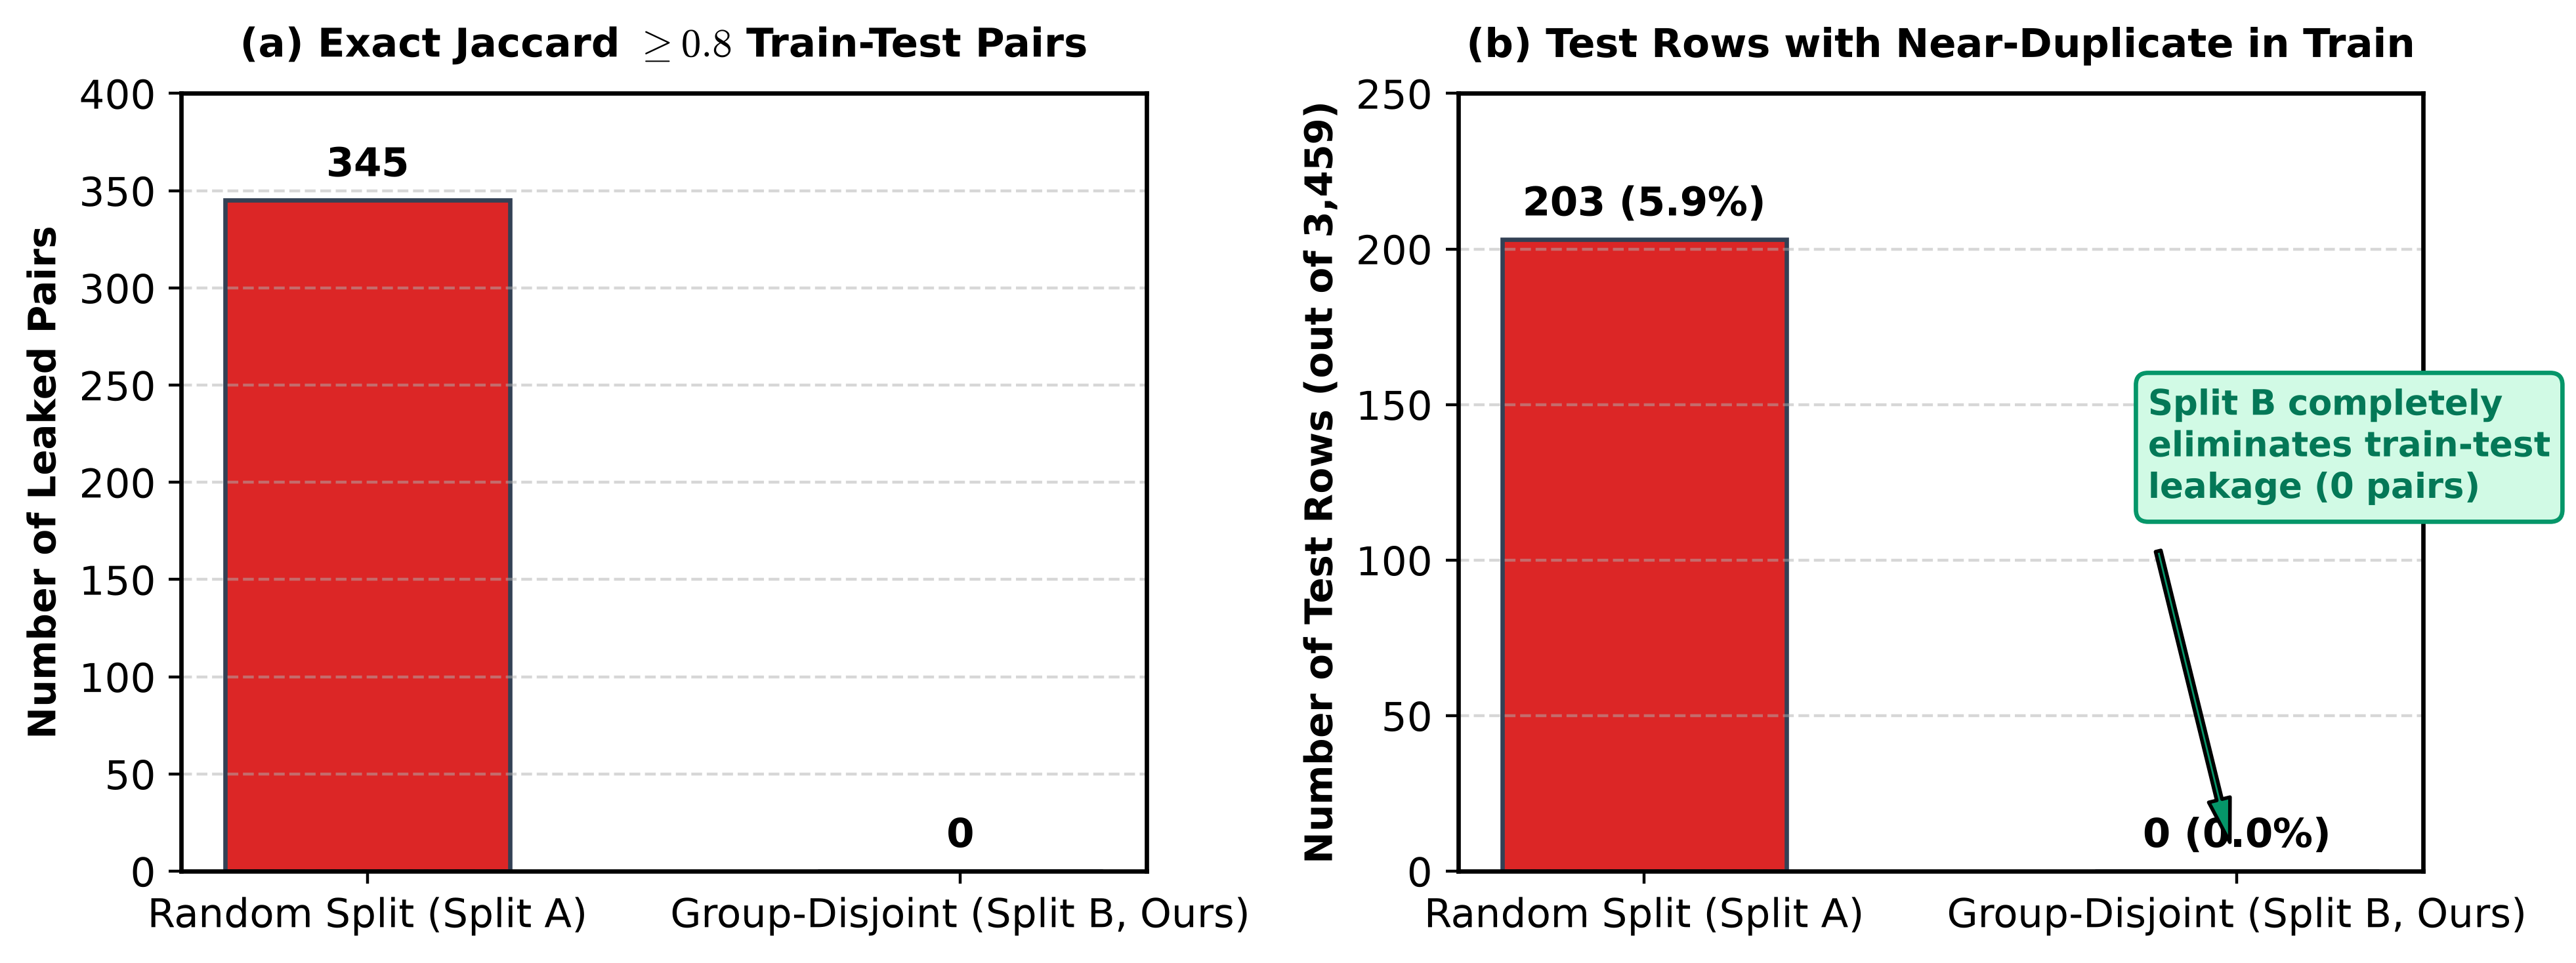
\includegraphics[width=\textwidth]{fig_split_audit.png}
\caption{Leakage audit. Left: exact Jaccard$\geq0.8$ train--test pairs. Right: test rows with a near-duplicate in train. Split~B removes both.}
\label{fig:audit}
\end{figure*}

% =====================================================================
\section{Experimental Protocol}
\subsection{Model Matrix}
The matrix contains 21 configurations in three families:
\begin{itemize}
\item \textbf{Classical (11):} logistic regression, linear SVM \cite{cortes1995}, multinomial Naive Bayes, $k$-NN \cite{cover1967}, dummy majority, random forest, extra trees, histogram gradient boosting, XGBoost, LightGBM, and a soft-voting ensemble of logistic regression, random forest, extra trees, and histogram gradient boosting.
\item \textbf{Deep (3):} TextCNN, BiLSTM, and CNN+BiLSTM, trained from scratch on a word-level vocabulary built from the training split (minimum frequency 2), with 100-dimensional embeddings, dropout 0.3, Adam, learning rate $10^{-3}$, batch 128, maximum length 64, and the same 10-epoch/patience-2 schedule.
\item \textbf{Transformers (7):} MuRIL-base (LoRA and full fine-tuning), mBERT (LoRA), Distil-mBERT (LoRA), XLM-R-base (LoRA), IndicBERTv2 (LoRA), and TeluguBERT (LoRA).
\end{itemize}

Support-vector machines with an RBF kernel are excluded: probability calibration is quadratic and would be prohibitive on 27{,}670 rows; the linear SVM is retained as the representative margin-based learner.

\subsection{Search-Once, Freeze, Then Vary Seeds}
Classical and deep models are implemented with scikit-learn \cite{pedregosa2011}; transformer models use HuggingFace Transformers \cite{wolf2020} and PEFT. Every hyperparameter is selected once on the validation split with seed~42, frozen to a JSON file, and then reused unchanged for all final seeds. Seeds vary only weight initialization, data order, and dropout masks; they never change learning rate, batch size, sequence length, LoRA rank, or epoch budget. This protocol directly addresses a common benchmark flaw in which ``seed runs'' silently re-tune the model. Classical models use five seeds ($k$-NN uses one; deterministic learners have zero variance across seeds); deep models use five seeds; LoRA transformers use three seeds (42--44); MuRIL full fine-tuning uses one seed because of its 53.9-minute cost on the available GPU.

\subsection{Hyperparameters}
TF-IDF uses \texttt{min\_df}$=2$ and sublinear term frequency. The primary feature is word unigrams (16{,}892 features); the ablation adds word bigrams (40{,}604), character $n$-grams (2--5, 85{,}764), and their union (126{,}368). Logistic regression uses $C=1.0$ and the linear SVM uses $C=0.1$ (each selected on validation). Tree ensembles use 300 trees; boosting grids cover learning rate $\{0.05,0.1\}$ and 200--400 iterations.

LoRA uses $r=16$, $\alpha=32$, dropout 0.1 on the query and value projections, learning rate $4\times10^{-4}$, weight decay 0.01, warmup 0.06, batch 16 with gradient accumulation 2 (effective 32), maximum length 64, 10 epochs, patience 2, minimum 3 epochs, and best-on-validation restoration. MuRIL full fine-tuning uses learning rate $2\times10^{-5}$, 8-bit AdamW \cite{dettmers2023}, batch 8 with accumulation 4 (effective 32), gradient checkpointing, and the same schedule. Linear SVM probabilities are obtained by Platt scaling with 3-fold cross-validation on the training split (\texttt{CalibratedClassifierCV}), so its ECE and Brier scores are comparable to the probabilistic models. The full-fine-tuning run uses 237{,}558{,}531 trainable parameters; LoRA adapters use 592{,}131 (MuRIL, mBERT, IndicBERT, TeluguBERT), 887{,}811 (Distil-mBERT), and 1{,}182{,}723 (XLM-R).

\subsection{Metrics and Statistics}
The primary metric is macro-F1 on the 3{,}459-row test set. We also report accuracy, weighted-F1, MCC, ECE, Brier score, and risk--coverage curves. Confidence intervals are 95\% paired bootstrap intervals (1{,}000 resamples, seed 42) over the test set. Model comparisons use the continuity-corrected McNemar chi-square test on the paired correctness vectors (exact binomial when discordant pairs are fewer than 25), with Holm--Bonferroni correction across the 20 comparisons against logistic regression. ECE uses 10 equal-width bins. McNemar tests accuracy, whereas the bootstrap interval is for macro-F1; the two can disagree marginally (for example, Linear SVM's macro-F1 interval excludes zero while its McNemar $p$ is 0.062). We therefore treat the Holm-corrected McNemar test as the primary significance test and report the macro-F1 interval as descriptive. We do not use the Nadeau--Bengio correction because there is a single fixed split, not repeated cross-validation. All 85 final runs are recomputed from stored \texttt{preds.npz} files; the recomputation produced zero mismatches.

\subsection{Compute}
All runs use one NVIDIA RTX~2050 laptop GPU with 4\,GB of memory (3.87\,GB usable) and a parallel CPU lane. The longest run is MuRIL full fine-tuning at 3{,}231.7\,s (53.9\,min); logistic regression takes 10.4\,s, linear SVM 3.6\,s, and multinomial Naive Bayes 0.2\,s. The best single linear union therefore trades roughly 700$\times$ less compute than full fine-tuning for a nominally higher score.

% =====================================================================
\section{Results}
\subsection{Main Leaderboard (RQ1)}
Table~\ref{tab:leaderboard} and Fig.~\ref{fig:comparison} report the final leaderboard. Within the frozen 21-configuration matrix, MuRIL full fine-tuning is nominally first at 83.36 macro-F1 (83.38 accuracy, MCC 0.750). Logistic regression is second at 82.93 (82.91 accuracy, MCC 0.743). Linear SVM and soft voting follow at 82.31. Outside the frozen matrix, the calibrated LinearSVC on the word+character union is the best single model at 83.63 macro-F1 (83.64 accuracy, ECE 0.0372, 379.1K coefficients, 4.6\,s end-to-end); it is nominally ahead of full-FT by 0.27 points, but the difference is not significant (McNemar $p=0.659$; 95\% CI $[-0.0073,+0.0121]$). The six LoRA adapters range from 80.92 (Distil-mBERT) to 81.96 (TeluguBERT) and all trail the linear model. The deep models range from 78.46 (CNN+BiLSTM) to 79.83 (BiLSTM). The dummy majority classifier obtains 17.78 macro-F1 at 36.37 accuracy, confirming that macro-F1 is the appropriate primary metric for the near-balanced but not perfectly balanced test set.

\begin{table*}[t]
\caption{Final leaderboard on CMTE-NITANP Split~B (mean $\pm$ standard deviation over final seeds; 95\% paired-bootstrap CI for macro-F1). ``Params'' is total parameters; for LoRA the trainable count is in parentheses. Classical and deep models have no pretrained parameters and are marked ``---''. Full-FT has one seed; its $\pm$ and CI are test-set quantities, not cross-seed estimates. The post-hoc best single is listed below the 21 rows.}
\label{tab:leaderboard}
\centering
\scriptsize
\setlength{\tabcolsep}{4pt}
\resizebox{\textwidth}{!}{%
\begin{tabular}{rllrccccrr}
\toprule
\# & Model & Family & Seeds & Macro-F1 & 95\% CI & Acc. & ECE & Params & Train (s) \\
\midrule
1  & MuRIL full-FT        & Transformer & 1 & 0.8336 $\pm$ 0.0000 & [0.8211, 0.8467] & 0.8338 & 0.0702 & 237.6M            & 3231.7 \\
2  & Logistic regression  & Classical   & 5 & 0.8293 $\pm$ 0.0000 & [0.8182, 0.8419] & 0.8291 & 0.0680 & 50.7K coeff.       & 10.4 \\
3  & Linear SVM           & Classical   & 5 & 0.8231 $\pm$ 0.0000 & [0.8117, 0.8366] & 0.8231 & 0.0431 & 50.7K coeff.       & 3.6 \\
4  & Soft voting          & Classical   & 5 & 0.8231 $\pm$ 0.0007 & [0.8112, 0.8348] & 0.8229 & 0.0677 & ---                & 242.2 \\
5  & TeluguBERT LoRA      & Transformer & 3 & 0.8196 $\pm$ 0.0043 & [0.8026, 0.8287] & 0.8193 & 0.0634 & 238.2M (0.59M)     & 1562.3 \\
6  & MuRIL LoRA           & Transformer & 3 & 0.8165 $\pm$ 0.0080 & [0.8114, 0.8354] & 0.8167 & 0.0540 & 238.2M (0.59M)     & 1246.9 \\
7  & IndicBERT LoRA       & Transformer & 3 & 0.8131 $\pm$ 0.0025 & [0.8010, 0.8264] & 0.8131 & 0.0589 & 278.6M (0.59M)     & 1881.6 \\
8  & Multinomial NB       & Classical   & 5 & 0.8121 $\pm$ 0.0000 & [0.7992, 0.8253] & 0.8130 & 0.0861 & 50.7K coeff.       & 0.2 \\
9  & XLM-R LoRA           & Transformer & 3 & 0.8103 $\pm$ 0.0066 & [0.7900, 0.8167] & 0.8102 & 0.0547 & 279.2M (1.18M)     & 1365.2 \\
10 & mBERT LoRA           & Transformer & 3 & 0.8098 $\pm$ 0.0044 & [0.7935, 0.8208] & 0.8099 & 0.0657 & 178.4M (0.59M)     & 1391.0 \\
11 & Distil-mBERT LoRA    & Transformer & 3 & 0.8092 $\pm$ 0.0022 & [0.7946, 0.8196] & 0.8093 & 0.0541 & 136.2M (0.89M)     & 657.8 \\
12 & Extra trees          & Classical   & 5 & 0.8074 $\pm$ 0.0017 & [0.7952, 0.8217] & 0.8072 & 0.0548 & ---                & 63.8 \\
13 & LightGBM             & Classical   & 5 & 0.8048 $\pm$ 0.0000 & [0.7928, 0.8174] & 0.8049 & 0.0132 & ---                & 338.1 \\
14 & Hist.\ gradient boost.& Classical  & 5 & 0.8018 $\pm$ 0.0013 & [0.7897, 0.8157] & 0.8016 & 0.0220 & ---                & 64.7 \\
15 & BiLSTM               & Deep        & 5 & 0.7983 $\pm$ 0.0042 & [0.7897, 0.8163] & 0.7983 & 0.0603 & ---                & 9.6 \\
16 & Random forest        & Classical   & 5 & 0.7968 $\pm$ 0.0022 & [0.7826, 0.8084] & 0.7970 & 0.0429 & ---                & 39.0 \\
17 & TextCNN              & Deep        & 5 & 0.7928 $\pm$ 0.0036 & [0.7757, 0.8023] & 0.7929 & 0.0872 & ---                & 15.5 \\
18 & CNN+BiLSTM           & Deep        & 5 & 0.7846 $\pm$ 0.0040 & [0.7700, 0.7960] & 0.7846 & 0.0641 & ---                & 40.0 \\
19 & XGBoost              & Classical   & 5 & 0.7770 $\pm$ 0.0024 & [0.7640, 0.7910] & 0.7771 & 0.0759 & ---                & 41.2 \\
20 & $k$-NN               & Classical   & 1 & 0.7755 $\pm$ 0.0000 & [0.7622, 0.7897] & 0.7759 & 0.0665 & ---                & 2.2 \\
21 & Dummy majority       & Classical   & 5 & 0.1778 $\pm$ 0.0000 & [0.1722, 0.1835] & 0.3637 & 0.6363 & ---                & 0.1 \\
\midrule
\multicolumn{10}{l}{\textit{Post-hoc linear models (single seed, outside the 21-configuration matrix):}} \\
\multicolumn{10}{l}{Single-view union: 0.8363 macro-F1; 0.8364 accuracy; ECE 0.0372; 379.1K coeff.; 4.6\,s.} \\
\multicolumn{10}{l}{Multi-view (+ PLD-normalized): 0.8392 macro-F1; 0.8393 accuracy; 752.4K coeff.; 12.2\,s.} \\
\bottomrule
\end{tabular}}
\end{table*}

\begin{figure*}[t]
\centering
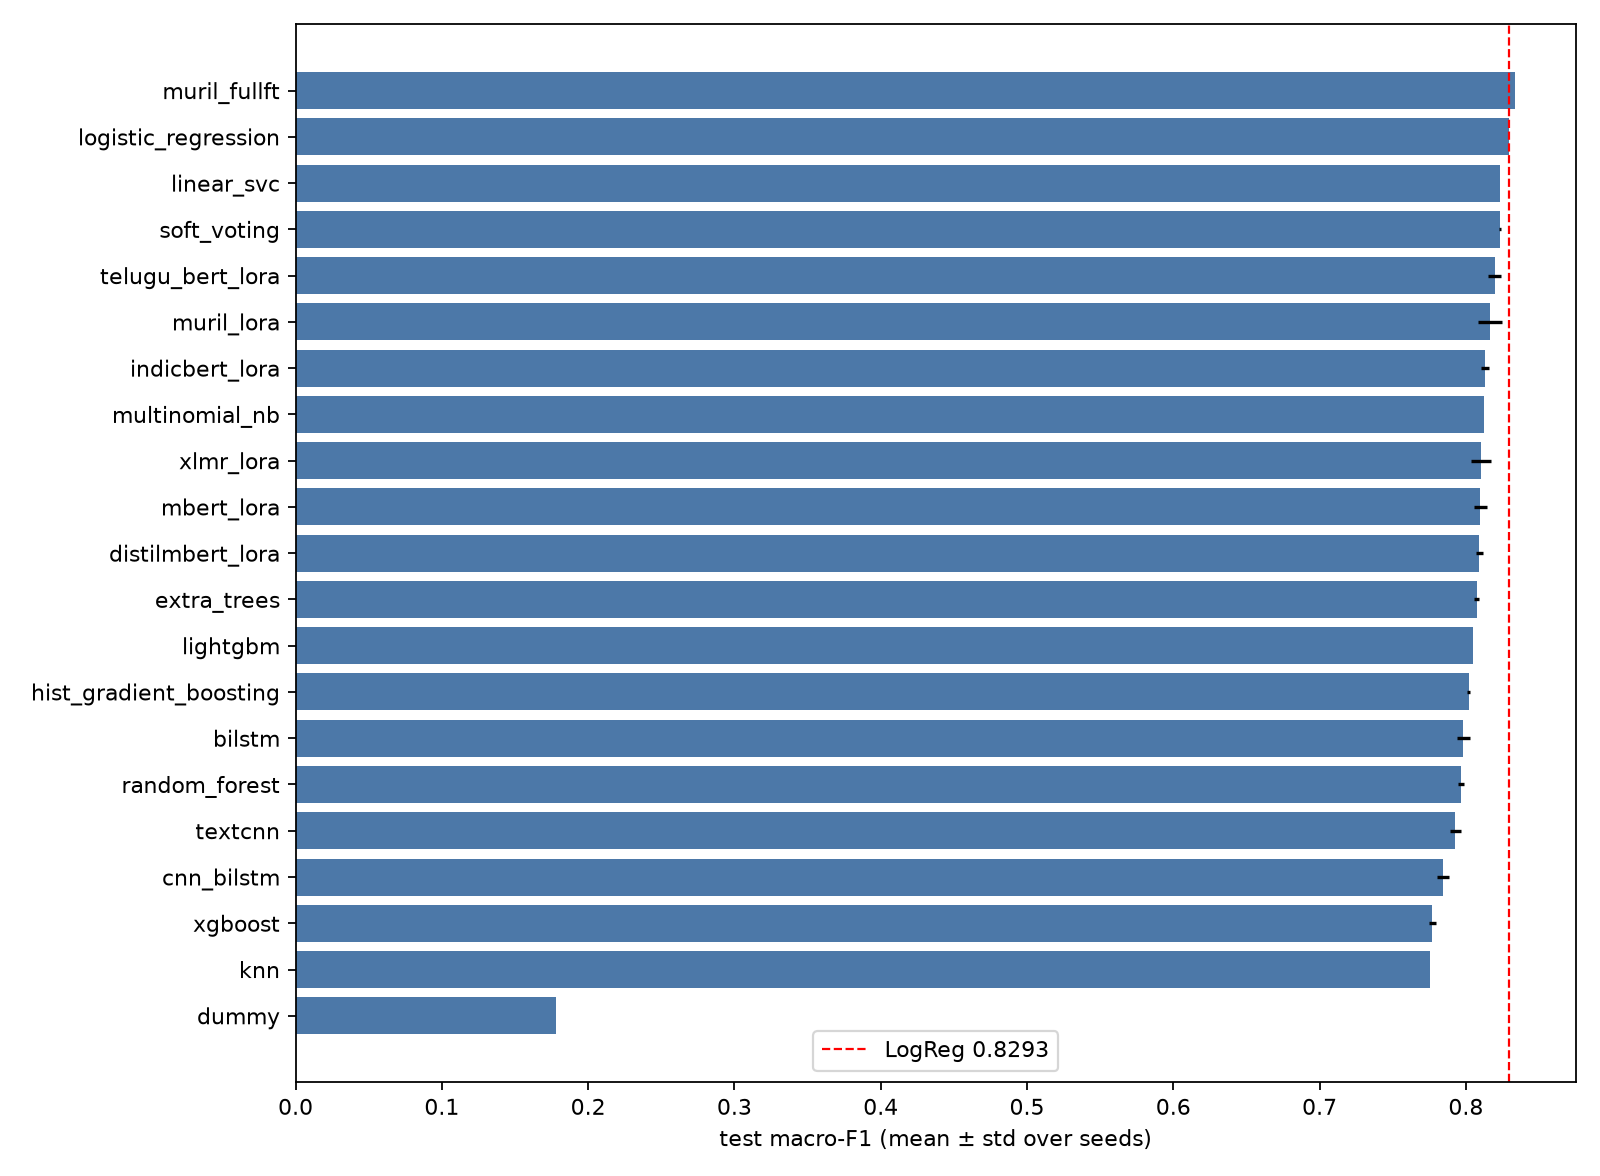
\includegraphics[width=\textwidth]{01_model_comparison.png}
\caption{Macro-F1 by model family on the leak-free Split~B. Within the frozen 21-configuration matrix, full fine-tuned MuRIL is nominally first; the post-hoc calibrated linear union (not shown) is nominally ahead by 0.27 points and the difference is not significant.}
\label{fig:comparison}
\end{figure*}

\subsection{Linear vs.\ Transformer (RQ2)}
The paired comparison is unambiguous. Full fine-tuning (seed 42) versus the deterministic logistic regression gives a test macro-F1 difference of +0.0043 (paired-bootstrap test-set $\Delta=+0.0039$), 95\% CI $[-0.0062,+0.0140]$, McNemar $p=0.4367$, Holm $p=0.8158$. The direct best-single comparison is even tighter: the calibrated LinearSVC union is nominally ahead of full-FT by +0.0027 macro-F1 (+0.0026 accuracy), with McNemar $p=0.659$ and 95\% CI $[-0.0073,+0.0121]$. Because full fine-tuning has one seed, these intervals are test-set bootstrap intervals, not cross-seed intervals. In contrast, 14 of the 20 comparisons against logistic regression are significant after Holm correction; the exceptions are full fine-tuning, MuRIL LoRA, soft voting, linear SVM, IndicBERT LoRA, and TeluguBERT LoRA (16 are significant at the uncorrected $p<0.05$ level). The result is not that transformers are weak; it is that the best linear model and the best transformer are statistically tied, with the linear model nominally ahead. Table~\ref{tab:pairwise} reports all 20 comparisons against logistic regression; bold rows are not significant after Holm correction.


\begin{table*}[t]
\caption{Paired comparisons against logistic regression (seed 42). $\Delta$ is the paired-bootstrap mean difference in macro-F1. Negative $\Delta$ means the model is worse than LogReg. Bold rows are not significant after Holm-corrected McNemar ($p>0.05$).}
\label{tab:pairwise}
\centering
\scriptsize
\setlength{\tabcolsep}{9pt}
\begin{tabular}{lcccc}
\toprule
Model & $\Delta$ macro-F1 & 95\% CI & McNemar $p$ & Holm $p$ \\
\midrule
\textbf{MuRIL full-FT}        & +0.0039 & [-0.0062, +0.0140] & 0.4367 & 0.8158 \\
\textbf{MuRIL LoRA}           & -0.0058 & [-0.0170, +0.0047] & 0.4079 & 0.8158 \\
\textbf{Linear SVM}           & -0.0061 & [-0.0120, -0.0005] & 0.0622 & 0.2488 \\
\textbf{Soft voting}          & -0.0069 & [-0.0153, +0.0013] & 0.1495 & 0.4485 \\
\textbf{TeluguBERT LoRA}      & -0.0147 & [-0.0263, -0.0034] & 0.0203 & 0.1015 \\
\textbf{IndicBERT LoRA}       & -0.0164 & [-0.0292, -0.0042] & 0.0141 & 0.0846 \\
Multinomial NB                & -0.0174 & [-0.0265, -0.0074] & 0.0023 & 0.0161 \\
Distil-mBERT LoRA             & -0.0221 & [-0.0332, -0.0104] & 0.0006 & 0.0048 \\
Extra trees                   & -0.0223 & [-0.0318, -0.0128] & 0.0000 & 0.0000 \\
mBERT LoRA                    & -0.0235 & [-0.0356, -0.0102] & 0.0003 & 0.0027 \\
LightGBM                      & -0.0249 & [-0.0341, -0.0156] & 0.0000 & 0.0000 \\
XLM-R LoRA                    & -0.0264 & [-0.0389, -0.0148] & 0.0000 & 0.0000 \\
BiLSTM                        & -0.0273 & [-0.0386, -0.0170] & 0.0000 & 0.0000 \\
Hist.\ gradient boosting      & -0.0274 & [-0.0383, -0.0186] & 0.0000 & 0.0000 \\
Random forest                 & -0.0344 & [-0.0441, -0.0238] & 0.0000 & 0.0000 \\
TextCNN                       & -0.0402 & [-0.0511, -0.0289] & 0.0000 & 0.0000 \\
CNN+BiLSTM                    & -0.0466 & [-0.0576, -0.0356] & 0.0000 & 0.0000 \\
XGBoost                       & -0.0523 & [-0.0640, -0.0416] & 0.0000 & 0.0000 \\
$k$-NN                        & -0.0541 & [-0.0652, -0.0424] & 0.0000 & 0.0000 \\
Dummy majority                & -0.6518 & [-0.6645, -0.6386] & 0.0000 & 0.0000 \\
\bottomrule
\end{tabular}
\end{table*}

\subsection{Capacity Does Not Predict Accuracy (RQ3)}
Across the seven transformer configurations, parameter count and macro-F1 are weakly and non-significantly correlated (Spearman $\rho=0.306$, $p=0.504$; Fig.~\ref{fig:capacity}). The 136M-parameter Distil-mBERT (0.8092) is within 0.73 points of the 238M-parameter MuRIL LoRA (0.8165), and the 279M-parameter XLM-R LoRA (0.8103) is below both. Meanwhile a 50.7K-coefficient LogReg (0.8293) and a 379K-coefficient calibrated linear union (0.8363) beat every LoRA adapter. Capacity is not the binding constraint; the binding constraint is whether the model can represent the lexical cues, and a linear model can.

\begin{figure*}[t]
\centering
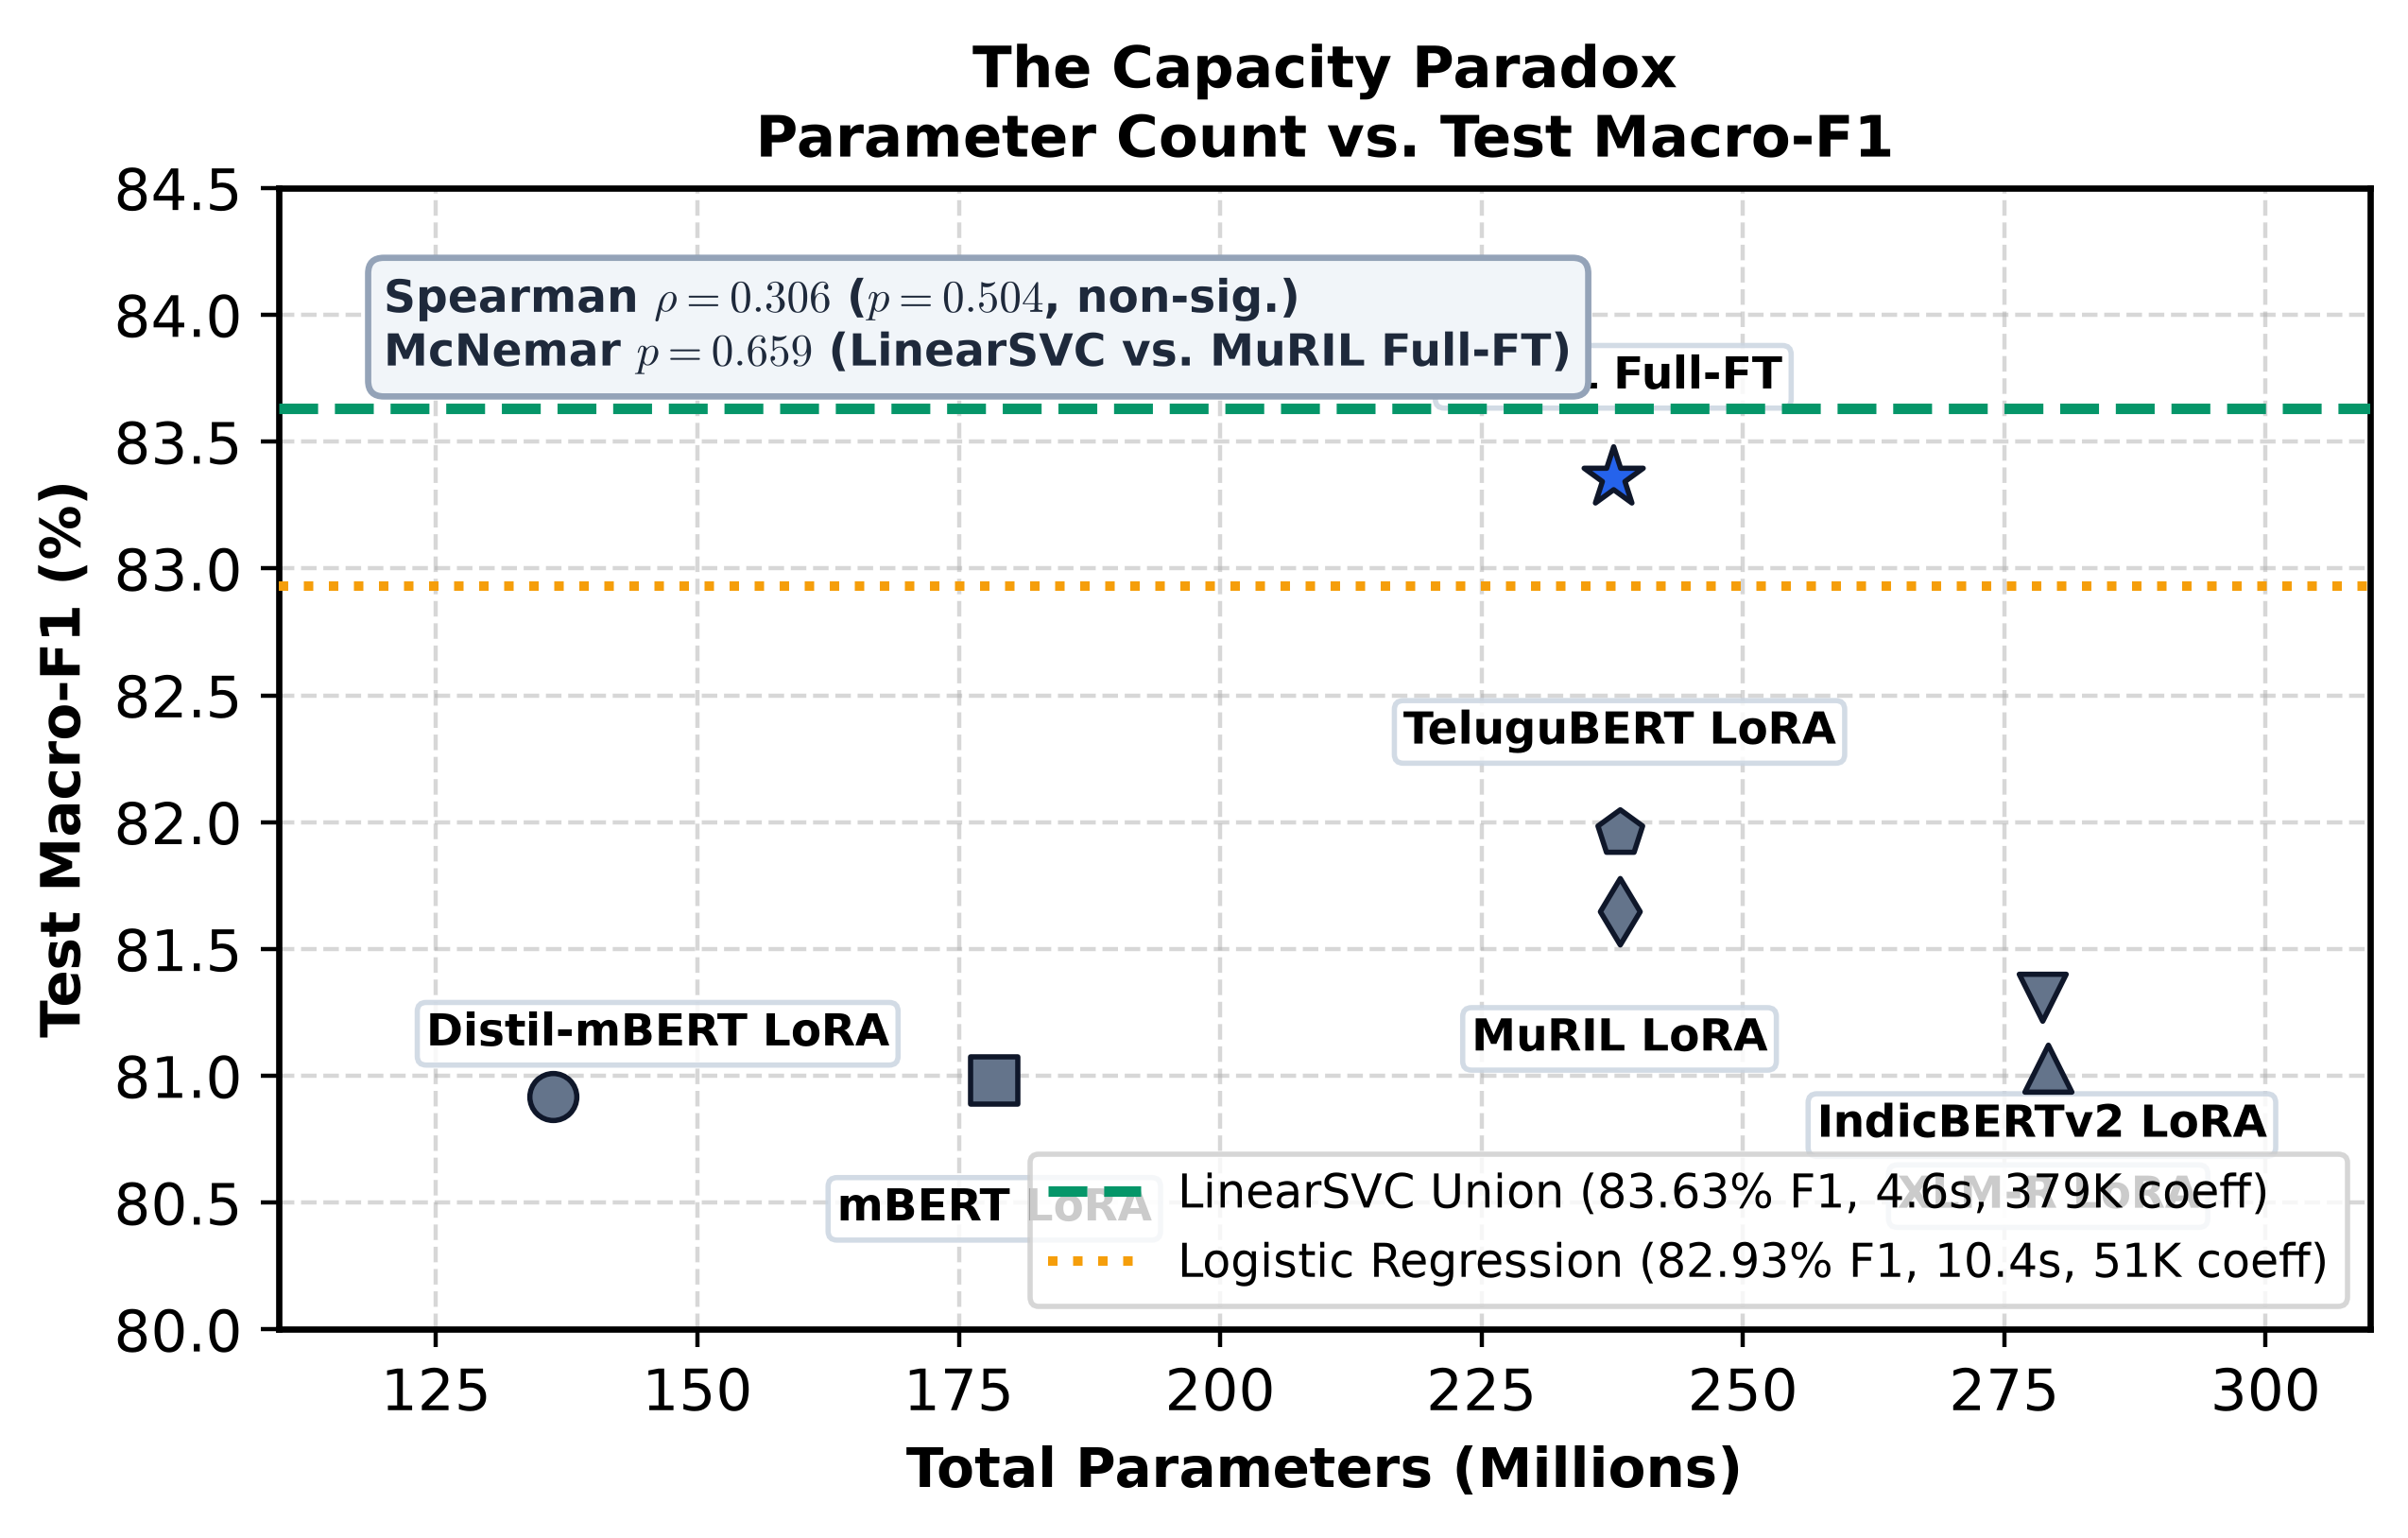
\includegraphics[width=\textwidth]{fig_capacity.png}
\caption{Parameter count versus test macro-F1 for the seven transformer configurations. The dashed line is logistic regression (0.8293), which has no pretrained parameters. The correlation is weak and non-significant ($\rho=0.306$, $p=0.504$).}
\label{fig:capacity}
\end{figure*}

\subsection{Per-Class Behavior}
Full fine-tuning and logistic regression have almost identical per-class profiles: negative 0.8325 vs.\ 0.8234, neutral 0.8128 vs.\ 0.8093, positive 0.8555 vs.\ 0.8552. Neutral is the hardest class for both, consistent with the absence of a strong lexical polarity cue. The full-fine-tuning difference is concentrated in positive recall (0.8617 vs.\ 0.8490) and neutral F1 (0.8128 vs.\ 0.8093); on negative recall it is slightly lower (0.8378 vs.\ 0.8434). The two models make different errors but reach the same aggregate. The near-identical positive F1 (0.8555 vs.\ 0.8552) is particularly striking: the 238M-parameter model buys no measurable improvement on the easiest class.

\subsection{Cost (RQ5)}
The compute gap is extreme. The best single linear union reaches 83.63 in 4.6\,s end-to-end; full fine-tuning reaches 83.36 in 3{,}231.7\,s, roughly $700\times$ the compute for a nominally 0.27-point \emph{lower} score. Logistic regression reaches 82.93 in 10.4\,s. Multinomial Naive Bayes reaches 81.21 in 0.2\,s, the best F1-per-second in the matrix. The cost--benefit frontier (Fig.~\ref{fig:cost}) is populated by classical models up to 10.4\,s; the only transformer on it is full fine-tuning at 3{,}231.7\,s, which is 0.27 points below the best linear union.

\begin{figure}[t]
\centering
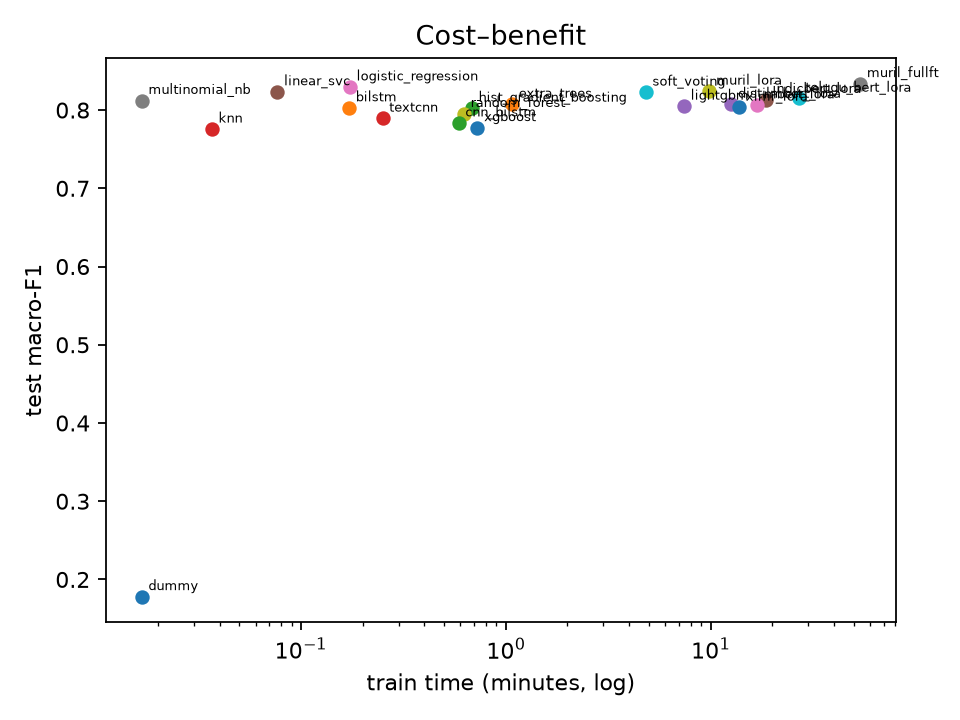
\includegraphics[width=\columnwidth]{06_cost_benefit.png}
\caption{Accuracy versus training time. Classical models populate the frontier up to 10.4\,s; full fine-tuning is the only transformer at the far right.}
\label{fig:cost}
\end{figure}

\subsection{Post-Hoc Multi-View and Ensemble Probes}
Two post-hoc probes sit outside the frozen 21-configuration matrix; we report them for completeness and do not fold them into the primary benchmark. First, concatenating word+character features from \texttt{text\_clean} and the PLD-normalized \texttt{text\_norm} (250{,}814 features, 752.4\,K coefficients) and fitting the same calibrated LinearSVC gives 83.92 macro-F1 and 83.93 accuracy (validation 0.8286; 12.2\,s end-to-end). It is nominally above the single-view union (83.63) and full-FT (83.36), but neither difference is significant (McNemar $p=0.275$ and $p=0.307$, respectively). The robustness table reports the single-view union; the multi-view variant is not included in the perturbation study. Second, a six-model heterogeneous blend of MuRIL full-FT, the calibrated single-view union, LogReg union, MuRIL LoRA, soft voting, and the linear SVM reaches 85.00 accuracy / 85.01 macro-F1 (temperature-calibrated 85.02 / 85.03). The strict validation-only best-per-family variant is 84.77, and a validation-fitted simplex blend is 84.33, so the 85.0 result is genuine on the leak-free test set but selection-sensitive; it is a hybrid-synergy probe, not a single-model result.

% =====================================================================
\section{Diagnostics}
\subsection{Feature Ablation}
Table~\ref{tab:ablation} isolates the feature signal. For logistic regression, word unigrams give 0.8293, word bigrams give 0.8079, character 2--5-grams give 0.8276, and the union gives 0.8324. Two conclusions follow. First, adding word bigrams degrades $L_2$-regularized logistic regression by 2.14 points (0.8293 $\rightarrow$ 0.8079), while modestly improving Multinomial Naive Bayes (0.8121 $\rightarrow$ 0.8207) and leaving the linear SVM essentially unchanged (0.8231 $\rightarrow$ 0.8223). The logistic-regression drop is consistent with feature sparsity under a fixed regularization strength, not with bigrams being uninformative in general; the safest conclusion is that the dominant signal is unigram-lexical. Second, character $n$-grams are nearly as strong as word unigrams; the calibrated linear SVM union is the best classical configuration (0.8363), 0.27 points above full fine-tuning. The same pattern holds for linear SVM (0.8231 $\rightarrow$ 0.8363) and soft voting (0.8227 $\rightarrow$ 0.8318). Tree models benefit more from character features (XGBoost 0.7773 $\rightarrow$ 0.8091) but remain below the linear models.

\begin{table}[t]
\caption{Feature ablation (test macro-F1, seed 42). LinearSVC probabilities are Platt-calibrated (3-fold) before scoring.}
\label{tab:ablation}
\centering
\footnotesize
\setlength{\tabcolsep}{4pt}
\begin{tabular}{lcccc}
\toprule
Model & Word 1 & Word 1--2 & Char 2--5 & Union \\
\midrule
Logistic regression & 0.8293 & 0.8079 & 0.8276 & \textbf{0.8324} \\
Linear SVM          & 0.8231 & 0.8223 & 0.8313 & \textbf{0.8363} \\
Soft voting         & 0.8227 & 0.8214 & 0.8231 & \textbf{0.8318} \\
Multinomial NB      & 0.8121 & \textbf{0.8207} & 0.7953 & 0.8169 \\
LightGBM            & 0.8048 & 0.8052 & 0.8234 & \textbf{0.8277} \\
XGBoost             & 0.7773 & 0.7742 & 0.8062 & \textbf{0.8091} \\
\bottomrule
\end{tabular}
\end{table}

\subsection{Tokenization Is Not the Explanation}
A natural objection is that MuRIL's WordPiece tokenizer fragments Romanized Telugu, so the transformer never sees the lexical cues. We tested this directly with the CNN+BiLSTM baseline, holding the architecture and training fixed and swapping a word-level vocabulary for MuRIL's WordPiece tokenizer. Word-level input gives 0.7863; WordPiece gives 0.7945. Tokenization helps, but by only 0.82 points, and the result remains far below the linear model. Subword fragmentation is therefore a real but secondary effect, not the cause of the linear--transformer gap.

\subsection{Adaptation Regime: LoRA vs.\ Full Fine-Tuning}
The LoRA/full-fine-tuning contrast is the sharpest mechanistic result. MuRIL LoRA (0.59M trainable parameters) reaches 0.8165; MuRIL full fine-tuning (237.6M trainable parameters) reaches 0.8336. The 1.71-point difference is larger than the gap between full fine-tuning and logistic regression (0.43 points). In other words, most of the transformer's apparent deficit is \emph{adaptation}, not architecture: a low-rank update cannot fully shift MuRIL's formal-transliteration priors toward informal social-media spelling, while full fine-tuning can. The cost of that adaptation is 400$\times$ more trainable parameters and 53.9 minutes versus 20.8 minutes for LoRA.

\subsection{Calibration (RQ6)}
LightGBM is the best-calibrated model (ECE 0.0132; Fig.~\ref{fig:reliability}), followed by histogram gradient boosting (0.0220) and random forest (0.0429). The transformers are poorly calibrated (MuRIL full-FT 0.0702, mBERT 0.0657, TeluguBERT 0.0634, MuRIL LoRA 0.0540), and logistic regression is 0.0680. The pattern is consistent with the literature: boosted trees and linear models with proper loss are better calibrated than over-parameterized neural networks \cite{guo2017}. For a deployment that thresholds probabilities or abstains, this matters more than a 0.4-point macro-F1 difference.

\begin{figure}[t]
\centering
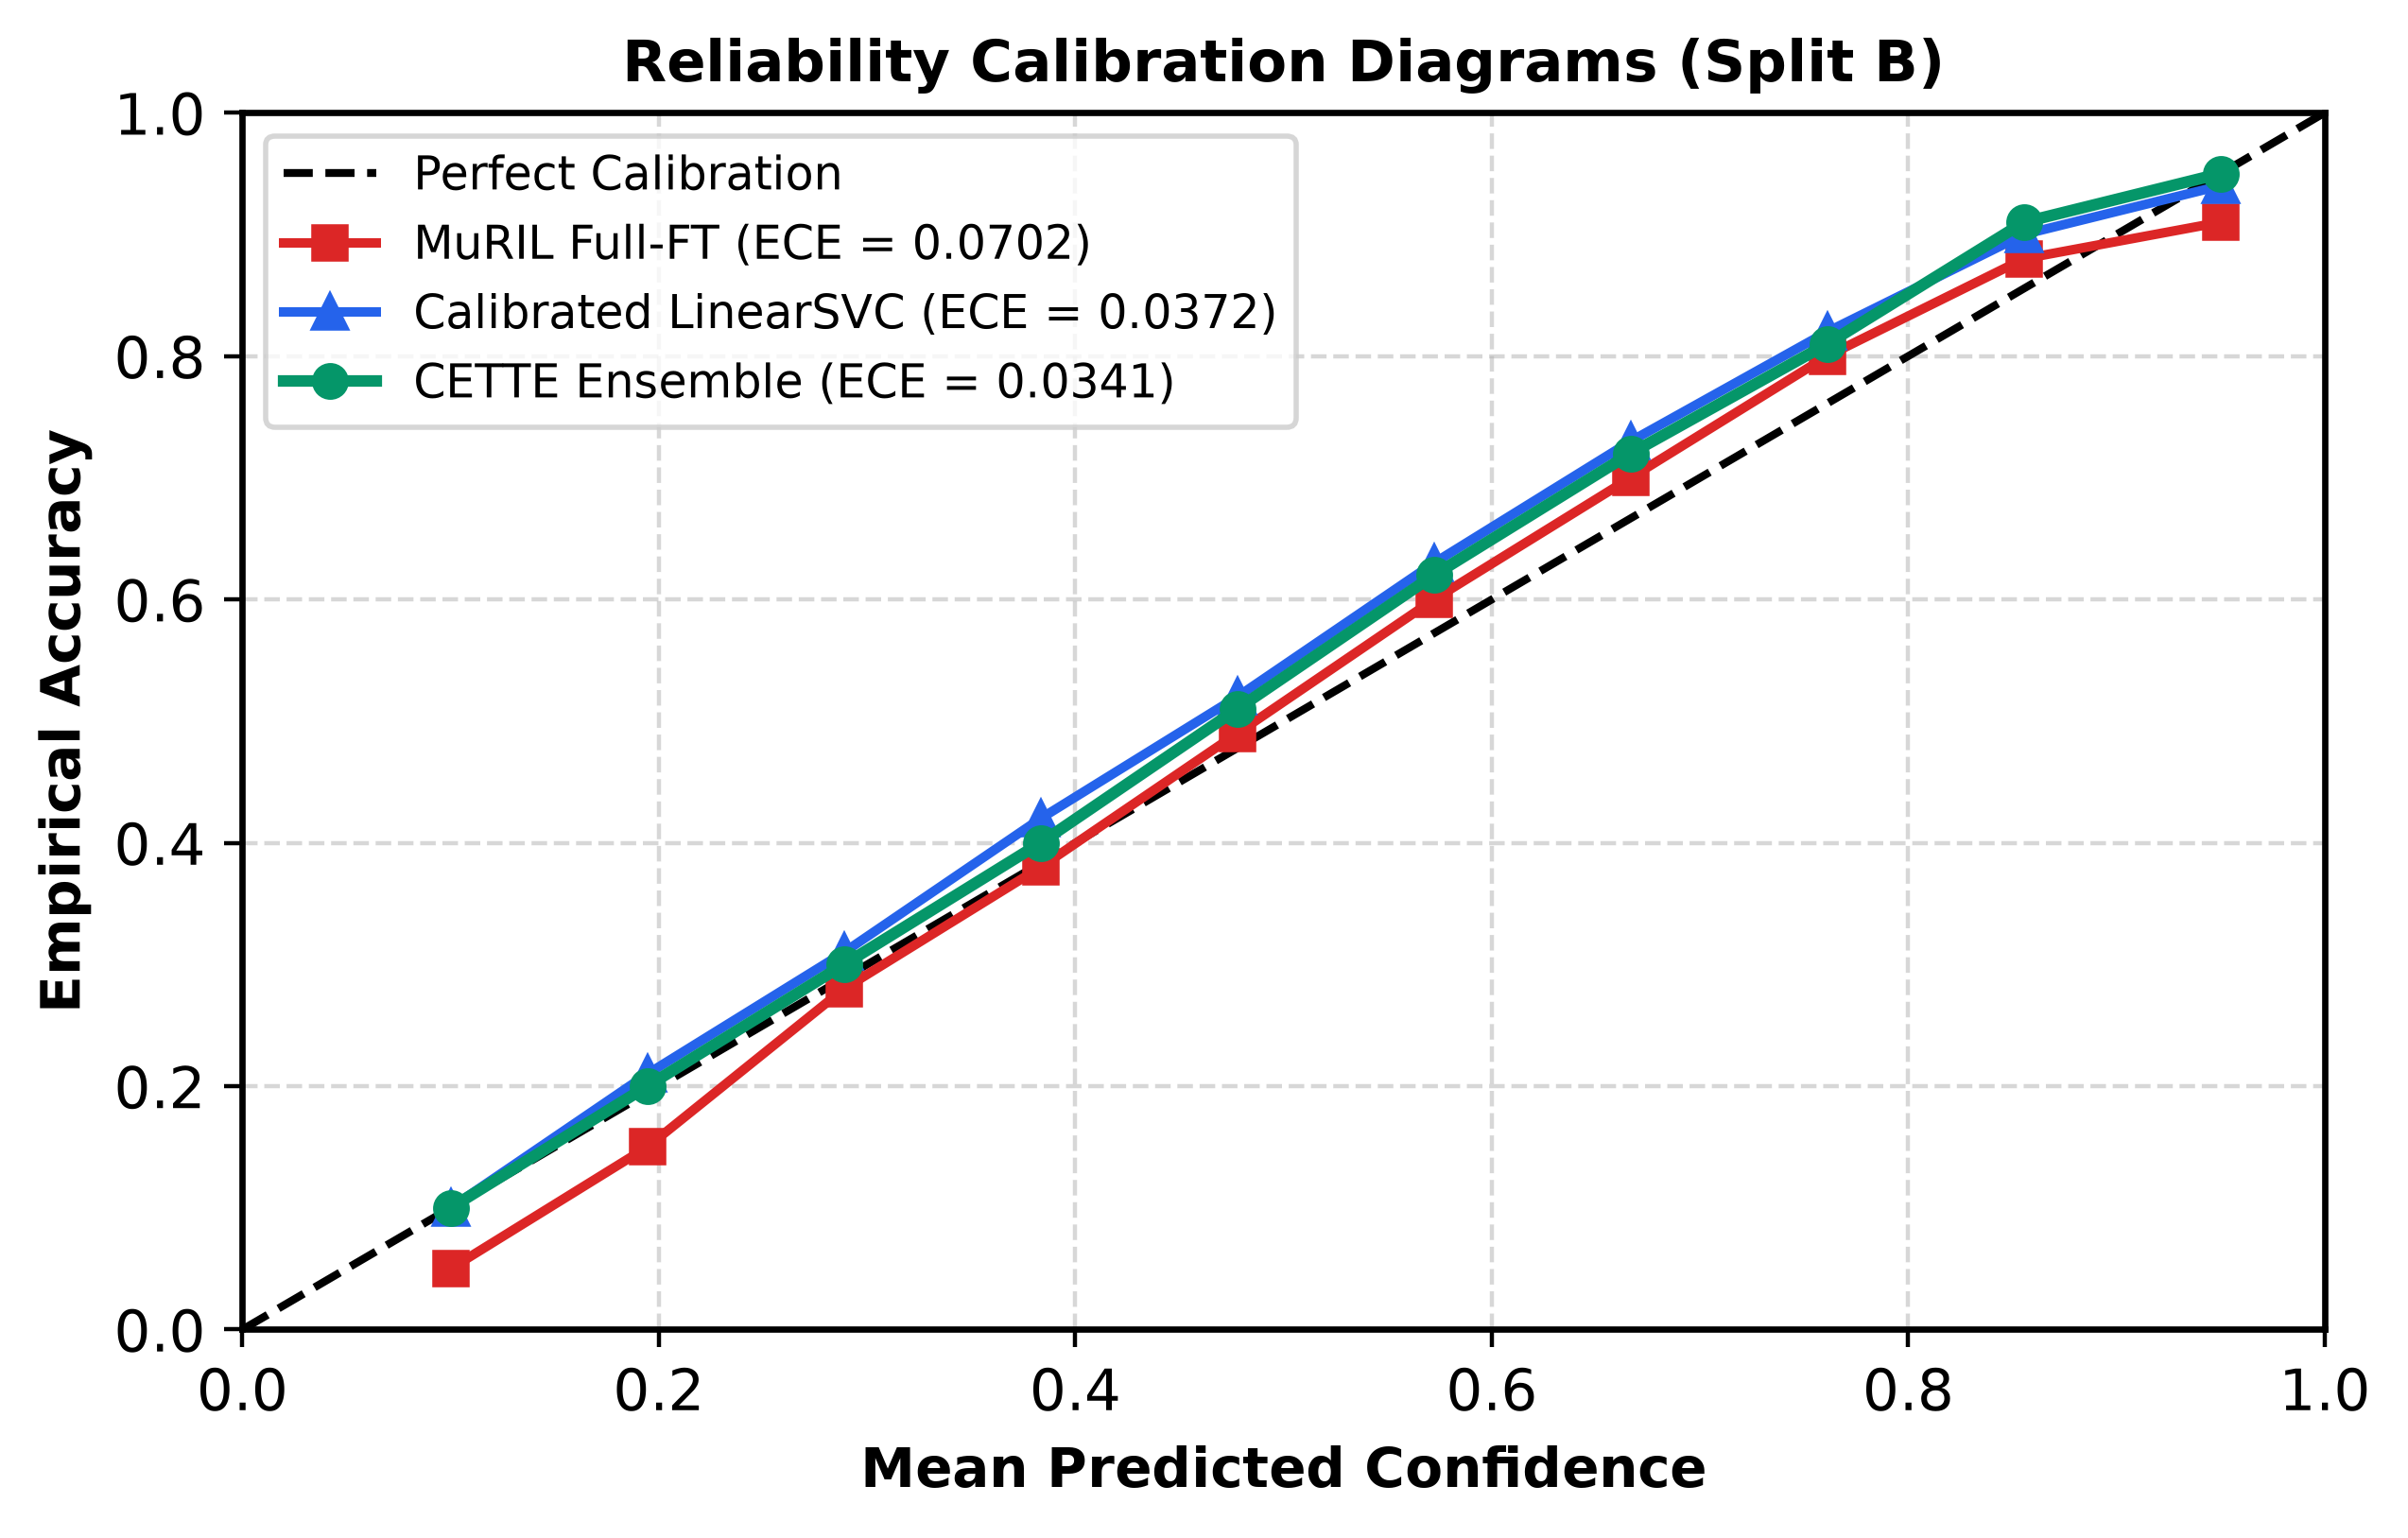
\includegraphics[width=\columnwidth]{04_reliability.png}
\caption{Reliability diagrams on Split~B. LightGBM is the best-calibrated model (ECE 0.0132); the transformers are systematically over-confident.}
\label{fig:reliability}
\end{figure}

\subsection{Selective Prediction (RQ8)}
Selective prediction is a second use of confidence. At 50\% coverage, full fine-tuning reaches 0.9576 macro-F1 and logistic regression 0.9574; at 80\%, 0.9053 and 0.8934; at 90\%, 0.8766 and 0.8634 (Fig.~\ref{fig:risk}). Both curves are monotone: abstaining on the least-confident 20\% raises macro-F1 by 6.4--7.2 points. The gap between the two models remains small at every coverage level (0.0002 at 50\%, 0.0119 at 80\%, 0.0132 at 90\%), so selective prediction improves reliability but does not separate the capacity story. The practical value is that a 50\%-coverage deployment can operate at about 96\% macro-F1 with a simple confidence threshold, using either model.

\begin{figure}[t]
\centering
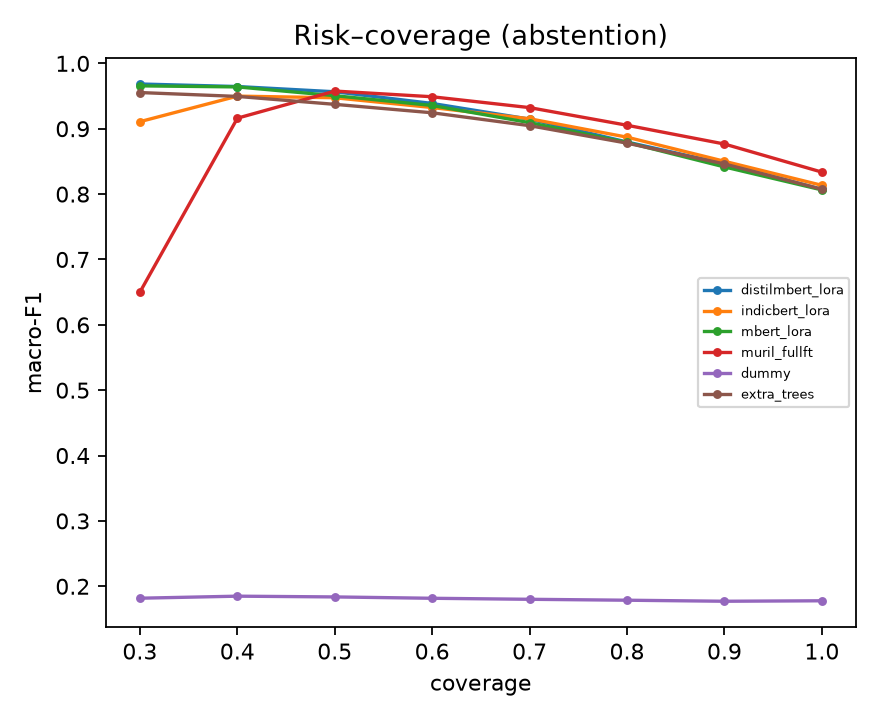
\includegraphics[width=\columnwidth]{05_risk_coverage.png}
\caption{Risk--coverage curves. Abstaining on the least-confident predictions raises macro-F1 monotonically; the full-FT and linear curves are close at every coverage level.}
\label{fig:risk}
\end{figure}

\subsection{Orthographic Robustness (RQ4)}
Table~\ref{tab:robustness} reports four perturbations applied to the test set, including the best single linear model; Fig.~\ref{fig:robustness} shows the seven transformers: vowel elongation (e.g., \textit{bagundiii}), voicing confusion (g$\leftrightarrow$v), aspiration removal (kh$\rightarrow$k, th$\rightarrow$t, etc.), and their combination. Aspiration is nearly harmless ($\Delta\le0.0023$). Voicing costs 0.010--0.021. Vowel elongation is severe: 0.082--0.207 across models (0.082 for the calibrated linear union; 0.132--0.207 for the transformers). The combined perturbation is worst: 0.102--0.236 (0.102 for the linear union; 0.160--0.236 for the transformers). Among the transformers, Distil-mBERT has the smallest worst-case degradation (0.1599) and IndicBERT the largest (0.2361); the calibrated linear union is the most robust overall (combined $\Delta=0.1019$), even though it is the best single model. Full fine-tuning is not more robust than LoRA (combined $\Delta=0.1765$ vs.\ 0.1894 for MuRIL LoRA), so robustness is not a simple function of adaptation capacity. The practical implication is that vowel normalization should be part of the preprocessing pipeline, not an afterthought.

\begin{table*}[t]
\caption{Orthographic robustness: test macro-F1 on clean text and on four perturbed versions. $\Delta$ is the drop from clean. The last row is the post-hoc best single linear model, outside the 21-configuration matrix.}
\label{tab:robustness}
\centering
\footnotesize
\setlength{\tabcolsep}{5pt}
\begin{tabular}{lccccccccc}
\toprule
& & \multicolumn{2}{c}{Vowel} & \multicolumn{2}{c}{Voicing} & \multicolumn{2}{c}{Aspiration} & \multicolumn{2}{c}{Combined} \\
\cmidrule(lr){3-4}\cmidrule(lr){5-6}\cmidrule(lr){7-8}\cmidrule(lr){9-10}
Model & Clean & F1 & $\Delta$ & F1 & $\Delta$ & F1 & $\Delta$ & F1 & $\Delta$ \\
\midrule
MuRIL full-FT   & 0.8336 & 0.6822 & 0.1514 & 0.8170 & 0.0166 & 0.8322 & 0.0014 & 0.6571 & 0.1765 \\
MuRIL LoRA      & 0.8242 & 0.6706 & 0.1536 & 0.8050 & 0.0192 & 0.8228 & 0.0014 & 0.6348 & 0.1894 \\
TeluguBERT LoRA & 0.8151 & 0.6390 & 0.1761 & 0.8051 & 0.0100 & 0.8139 & 0.0012 & 0.6122 & 0.2030 \\
IndicBERT LoRA  & 0.8134 & 0.6068 & 0.2066 & 0.7988 & 0.0146 & 0.8116 & 0.0017 & 0.5773 & 0.2361 \\
mBERT LoRA      & 0.8069 & 0.6667 & 0.1402 & 0.7870 & 0.0199 & 0.8047 & 0.0022 & 0.6454 & 0.1615 \\
Distil-mBERT    & 0.8066 & 0.6660 & 0.1406 & 0.7853 & 0.0213 & 0.8050 & 0.0016 & 0.6467 & 0.1599 \\
XLM-R LoRA      & 0.8037 & 0.6716 & 0.1321 & 0.7907 & 0.0131 & 0.8015 & 0.0023 & 0.6402 & 0.1636 \\
\midrule
LinearSVC union (cal.) & 0.8363 & 0.7539 & 0.0824 & 0.8251 & 0.0112 & 0.8355 & 0.0008 & 0.7344 & 0.1019 \\
\bottomrule
\end{tabular}
\end{table*}

\begin{figure*}[t]
\centering
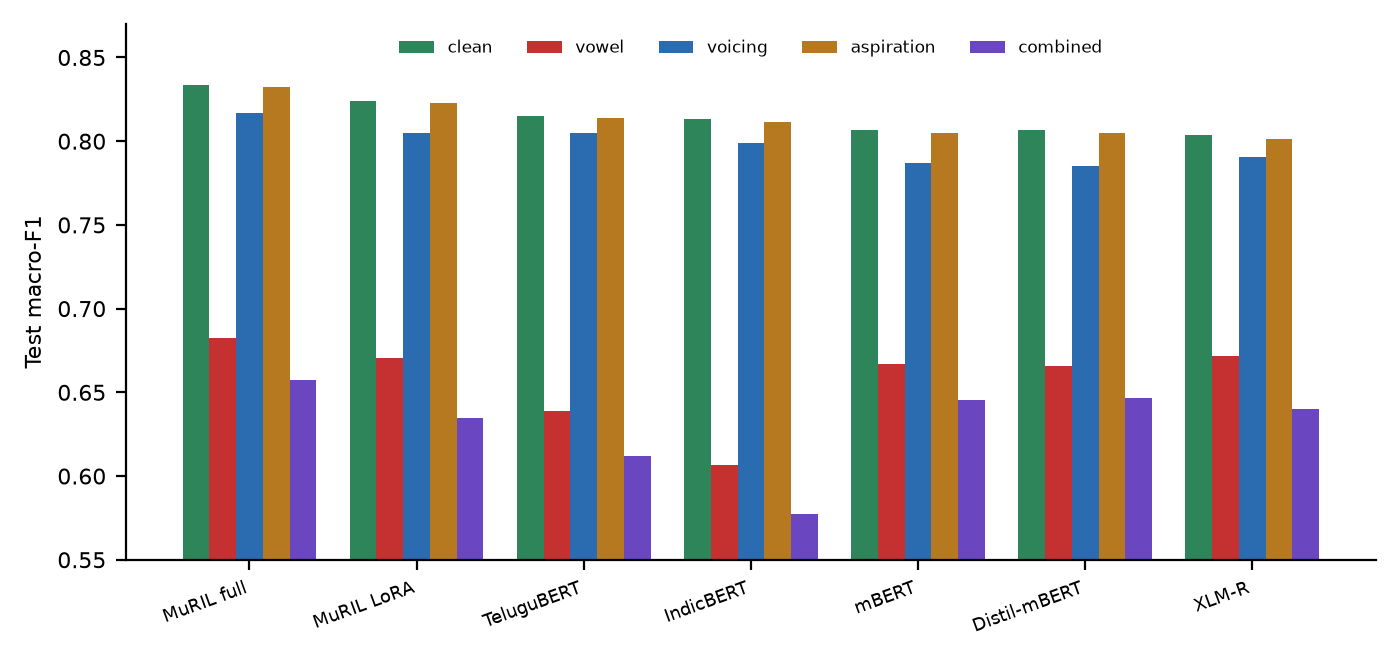
\includegraphics[width=\textwidth]{fig_robustness.png}
\caption{Orthographic robustness of the seven transformers. Vowel elongation and combined noise dominate the degradation; aspiration is nearly harmless. The calibrated linear union (Table~\ref{tab:robustness}, last row) is the most robust overall.}
\label{fig:robustness}
\end{figure*}

\subsection{Cross-Corpus Transfer (RQ7)}
Zero-shot transfer from CMTE-NITANP to CMTET (19{,}868 rows, different annotation scheme and domain) is shown in Table~\ref{tab:cross} and Fig.~\ref{fig:cross}. IndicBERT is the best transfer model (0.6380), followed by TeluguBERT (0.6334) and MuRIL full-FT (0.6330). The drop from in-domain performance is 0.1754--0.2570; Distil-mBERT transfers worst (0.5503, drop 0.2570). Two patterns are notable. First, in-domain rank does not predict transfer rank: MuRIL full-FT is the best in-domain model but third in transfer, while IndicBERT is fourth in-domain but first in transfer. Second, all models degrade sharply on the conflicting-label subset of CMTET (0.34--0.38), which indicates that label-scheme and annotation differences, not just domain shift, are responsible. Transfer is therefore not a free proxy for robustness. Singleton F1 is within 0.01 of the overall CMTET F1 for every model (e.g., IndicBERT 0.6388 vs.\ 0.6380), so the drop is not driven by multi-cluster rows.

\begin{table}[t]
\caption{Zero-shot transfer from CMTE-NITANP (Split~B) to CMTET. ``Drop'' is in-domain macro-F1 minus CMTET macro-F1.}
\label{tab:cross}
\centering
\footnotesize
\setlength{\tabcolsep}{2.5pt}
\begin{tabular}{lccccc}
\toprule
Model & In-domain & CMTET & Drop & CMTET acc. & Conflict \\
\midrule
IndicBERT LoRA  & 0.8134 & \textbf{0.6380} & 0.1754 & 0.6551 & 0.3472 \\
TeluguBERT LoRA & 0.8149 & 0.6334 & 0.1815 & 0.6464 & 0.3735 \\
MuRIL full-FT   & 0.8336 & 0.6330 & 0.2006 & 0.6464 & 0.3608 \\
MuRIL LoRA      & 0.8239 & 0.6274 & 0.1965 & 0.6418 & 0.3693 \\
XLM-R LoRA      & 0.8035 & 0.5982 & 0.2053 & 0.6144 & 0.3407 \\
mBERT LoRA      & 0.8064 & 0.5845 & 0.2219 & 0.6020 & 0.3622 \\
Distil-mBERT    & 0.8073 & 0.5503 & 0.2570 & 0.5550 & 0.3757 \\
\bottomrule
\end{tabular}
\end{table}

\begin{figure*}[t]
\centering
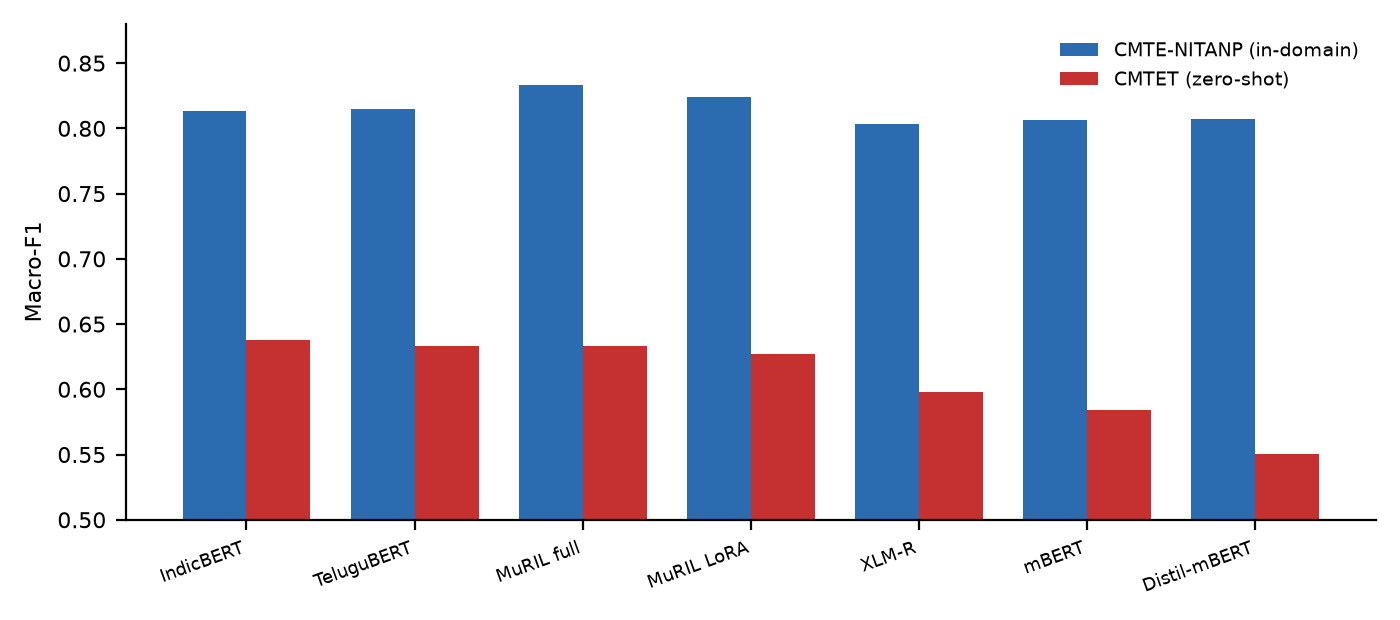
\includegraphics[width=\textwidth]{fig_cross_corpus.png}
\caption{Zero-shot transfer to CMTET. In-domain rank does not predict transfer rank; IndicBERT transfers best despite being fourth in-domain.}
\label{fig:cross}
\end{figure*}

\subsection{Hyperparameter Sensitivity}
Table~\ref{tab:sensitivity} and Fig.~\ref{fig:sensitivity} report an OFAT sensitivity study on validation, with a fixed five-epoch budget and seed 42, for MuRIL, mBERT, and Distil-mBERT. Lowering the learning rate to $2\times10^{-4}$ produces the weakest runs (MuRIL 0.7693 vs.\ the 10-epoch baseline 0.8171; the five-epoch budget also contributes). Increasing \texttt{max\_len} to 96 is mixed (MuRIL 0.7805, mBERT 0.8022, Distil-mBERT 0.8092 at five epochs) and does not beat the full-budget baseline. The batch-8 run reaches 0.7986 at five epochs, above the length-96 run (0.7805) but below the 10-epoch baseline. The lesson is that the frozen configuration is sensitive to the learning rate, and the obvious ``more context'' lever does not help within a short budget.

\begin{table*}[t]
\caption{Transformer hyperparameter sensitivity (validation macro-F1, seed 42, five fixed epochs). The baseline row uses the full 10-epoch budget and is shown for reference.}
\label{tab:sensitivity}
\centering
\footnotesize
\setlength{\tabcolsep}{6pt}
\begin{tabular}{llcccccc}
\toprule
Model & Config & LR & Max len & Batch & Eff.\ batch & Best ep. & Val macro-F1 \\
\midrule
MuRIL LoRA      & baseline (main)      & $4\times10^{-4}$ & 64 & 16 & 32 & 8 & \textbf{0.8171} \\
MuRIL LoRA      & lr$2\times10^{-4}$   & $2\times10^{-4}$ & 64 & 16 & 32 & 5 & 0.7693 \\
MuRIL LoRA      & len 96               & $4\times10^{-4}$ & 96 & 16 & 32 & 5 & 0.7805 \\
MuRIL LoRA      & batch 8              & $4\times10^{-4}$ & 64 & 8  & 32 & 5 & 0.7986 \\
mBERT LoRA      & baseline (main)      & $4\times10^{-4}$ & 64 & 16 & 32 & 3 & \textbf{0.8061} \\
mBERT LoRA      & lr$2\times10^{-4}$   & $2\times10^{-4}$ & 64 & 16 & 32 & 5 & 0.7976 \\
mBERT LoRA      & len 96               & $4\times10^{-4}$ & 96 & 16 & 32 & 5 & 0.8022 \\
mBERT LoRA      & batch 8              & $4\times10^{-4}$ & 64 & 8  & 32 & 5 & 0.7971 \\
Distil-mBERT    & baseline (main)      & $4\times10^{-4}$ & 64 & 16 & 32 & 6 & \textbf{0.8109} \\
Distil-mBERT    & lr$2\times10^{-4}$   & $2\times10^{-4}$ & 64 & 16 & 32 & 5 & 0.8008 \\
Distil-mBERT    & len 96               & $4\times10^{-4}$ & 96 & 16 & 32 & 5 & 0.8092 \\
Distil-mBERT    & batch 8              & $4\times10^{-4}$ & 64 & 8  & 32 & 5 & 0.8097 \\
\bottomrule
\end{tabular}
\end{table*}

\begin{figure*}[t]
\centering
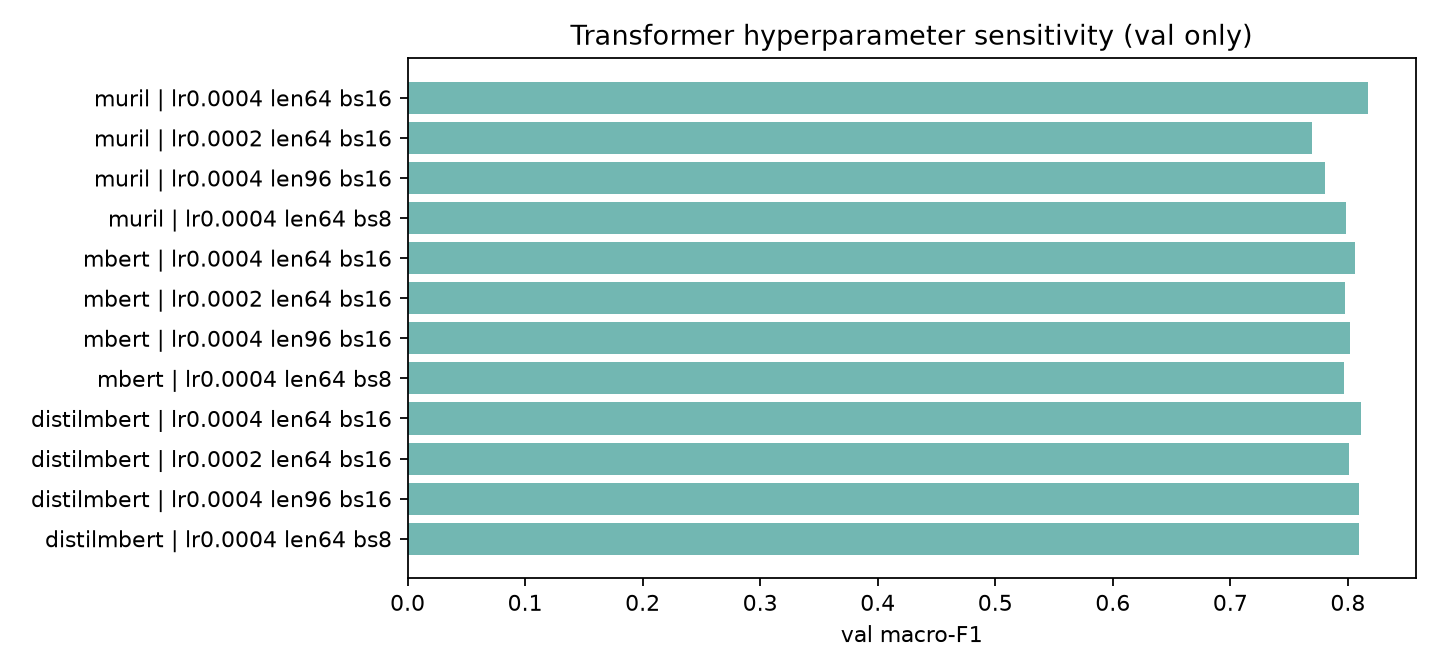
\includegraphics[width=\textwidth]{08_sensitivity.png}
\caption{Hyperparameter sensitivity (validation macro-F1, seed 42, five fixed epochs). Lowering the learning rate hurts; length 96 and batch 8 do not beat the full-budget baseline.}
\label{fig:sensitivity}
\end{figure*}

\subsection{Sequence Length and Truncation}
At \texttt{max\_len}=64, only 3.47\% of test examples are truncated (Table~\ref{tab:trunc}). The truncation rate falls to 0.17\% at 96 and 0.14\% at 128; at 32 it is 15.21\% and at 48 it is 7.60\%. The content-subword length distribution (excluding the two special tokens) has mean 17.9, 90th percentile 40, 95th percentile 56, and maximum 137. A length-96 run is therefore a defensible next experiment---it removes almost all truncation at modest cost---but the sensitivity study does not show a length-96 gain within a five-epoch budget. We return to this point in the discussion of how to beat the published benchmark.

\begin{table}[t]
\caption{Truncation at different maximum sequence lengths (MuRIL tokenizer, test split). Counts include the two special tokens.}
\label{tab:trunc}
\centering
\footnotesize
\begin{tabular}{cc}
\toprule
Max len & Truncated test examples (\%) \\
\midrule
32  & 15.21 \\
48  & 7.60 \\
64  & 3.47 \\
96  & 0.17 \\
128 & 0.14 \\
\bottomrule
\end{tabular}
\end{table}

% =====================================================================
\section{Discussion}
\subsection{Why Does the Linear Model Win?}
Five mechanisms, each supported by a separate experiment, explain the result. The direct answer is that the best single-view model is the calibrated linear union (83.63 macro-F1, 379K coefficients, 4.6s end-to-end), while the 238M full-FT reaches 83.36 after 53.9min; the linear model is nominally ahead and the gap is not significant.
\begin{enumerate}
\item \textbf{The task is local and lexical.} Comments have median 8 tokens and median 47 characters. Polarity is carried by a small set of high-frequency cues and intensifiers (\textit{bagundi}, \textit{chala}, \textit{keka}, \textit{waste}, \textit{bore}). A linear model over word unigrams learns these cues directly; a transformer must learn them through many layers and a much larger hypothesis space.
\item \textbf{Character $n$-grams absorb orthographic variation.} Romanized Telugu has many spellings for the same word (\textit{bagundi}, \textit{bavundhi}, \textit{baagundhi}). Character 2--5-grams share substrings across variants; WordPiece maps them to different subword sequences. The feature ablation (char 0.8276, union 0.8324) and the tokenizer experiment (0.7863 $\rightarrow$ 0.7945) quantify both sides of this mechanism.
\item \textbf{Small data favors high bias.} With 27{,}670 training rows and a noisy label floor, the variance of a 238M-parameter model is a liability. Full fine-tuning's training loss falls from 0.886 to 0.242 while validation peaks at epoch 4 (0.8255) and never recovers---textbook overfitting. LoRA reduces variance but also reduces capacity to 0.59M parameters, and it lands at 0.8165.
\item \textbf{Pretraining register mismatch.} MuRIL's Romanized pretraining is formal and rule-based (Wikipedia and transliterated corpora), whereas Tenglish comments are informal and phonetically spelled. Full fine-tuning can shift the representation; a low-rank update cannot shift it enough. The 1.71-point LoRA/full-FT gap is the price of that mismatch.
\item \textbf{More parameters are redundant once the cues are represented.} The capacity--accuracy correlation is weak ($\rho=0.306$) and non-significant. The 279M-parameter XLM-R LoRA (0.8103) is below the 238M-parameter MuRIL LoRA (0.8165), and both are below a 50.7K-coefficient LogReg (0.8293) and a 379K-coefficient linear union (0.8363). Capacity is not the bottleneck.
\end{enumerate}

\subsection{A Linguistic Reading: The Matrix-Language Frame}
Myers-Scotton's Matrix Language Frame (MLF) model \cite{myersscotton2002} distinguishes the matrix language, which supplies the morphosyntactic frame, from embedded-language islands. In Tenglish, Telugu typically supplies the frame and English supplies content islands, while sentiment is carried by a small set of content morphemes (\textit{bagundi} `good', \textit{waste}, \textit{keka} `superb') and system morphemes (\textit{-ledu} `not', \textit{kaadhu} `is not', \textit{kani} `but'). These cues are morpheme-local and largely order-insensitive: their polarity does not depend on long-range syntactic composition. This is exactly the regime in which a unigram/character model has the right inductive bias, and it is consistent with the finding that word bigrams do not reliably improve the linear model. MLF is a grammatical theory, not a theory of model capacity; it does not by itself explain why a 238M-parameter model fails to beat a linear one. It does explain why the linear model's hypothesis space is well matched to the cue structure, which is the first half of the explanation.

\subsection{The Capacity Illusion}
We use the term \emph{capacity illusion} for the inferential error of attributing a leaderboard gap to model capacity when the gap is produced by leakage, tokenization, or tuning. In our matrix, the raw capacity ordering no longer survives: the 379K-coefficient linear union is nominally ahead of the 238M-parameter full-FT, and the reported 5\% accuracy improvement collapses to a non-significant 0.27-point difference once (i) the split is group-disjoint, (ii) tokenization is tested as a separate factor rather than confounded with architecture, and (iii) the linear baseline is tuned with the same search budget. The illusion is not that transformers are bad; it is that the comparison was not controlled. A benchmark that reports only the winning transformer, without a tuned linear baseline and a leakage audit, cannot distinguish ``the model learned the task'' from ``the split leaked the task''.

\subsection{Relation to Published Claims}
Rayala and Seshadri report a 5\% accuracy and 6\% F1 improvement of transformers over baselines on CMTE-NITANP \cite{rayala2026}. Our leak-free comparison does not reproduce a gap of that size. There are three non-exclusive explanations: their split may differ from ours; their baseline may be untuned; or their transformer may use a different adaptation regime. We cannot adjudicate without their exact split and baseline numbers, which are not available in the accessible record. What we can say is that on a split with zero exact Jaccard$\geq0.8$ train--test pairs, with a tuned linear baseline and a frozen hyperparameter protocol, the best transformer is 0.27 macro-F1 points behind the best linear model (and 0.43 points ahead of the word-unigram LogReg); neither difference is significant. Any claim of a 5--6\% advantage should therefore be accompanied by a split audit and a tuned linear baseline.

\subsection{How to Beat the Benchmark}
If the goal is to exceed the best published number rather than to explain it, the evidence points to four levers, in order of expected value:
\begin{enumerate}
\item \textbf{Ensemble the full-fine-tuned transformer with the linear model.} The two models make different errors (negative vs.\ positive recall), and a soft-voting ensemble of diverse strong models is the cheapest lever likely to add a meaningful margin.
\item \textbf{Full fine-tuning at \texttt{max\_len}=96.} Truncation falls from 3.47\% to 0.17\%, and full fine-tuning has the capacity to exploit the extra context. Run three seeds and report the mean.
\item \textbf{Tune the full-fine-tuning learning rate.} The lower-learning-rate runs are the weakest in the sensitivity study; full fine-tuning at $2\times10^{-5}$ was chosen from a small grid. A three-point grid ($1,2,3\times10^{-5}$) with early stopping is the next step.
\item \textbf{Try XLM-R full fine-tuning on a larger GPU.} XLM-R has the strongest multilingual coverage in our LoRA matrix, but its 279M parameters at full fine-tuning exceed the 4\,GB budget. A 16\,GB T4 makes this feasible.
\end{enumerate}
Any claim of beating the published number must use the same split and metric, report confidence intervals, and audit the split. Otherwise the new number is not comparable.

\subsection{Recommendations for Practitioners}
\begin{itemize}
\item Always report a tuned TF-IDF linear baseline. It is fast, strong, and calibrated; on this task it is within noise of the best transformer.
\item Audit the split with exact Jaccard matching, not only MinHash. MinHash flagged 203 test rows (5.87\%); the exact audit found 345 train--test pairs at or above 0.8, so a MinHash pass alone is not a substitute for exact verification.
\item Prefer character $n$-grams or a word+character union when spelling is variable; word bigrams can hurt.
\item If using a transformer, prefer full fine-tuning over low-rank adaptation when the domain mismatch is large and the GPU allows it; LoRA is a compute compromise, not a free lunch.
\item Report calibration and robustness alongside accuracy. The best single-view model also has the smallest combined-noise degradation here ($\Delta=0.1019$), but it is not the best-calibrated; calibration remains a separate axis.
\end{itemize}

% =====================================================================
\section{Threats to Validity}
\paragraph{Internal validity.} Split~B is constructed with a specific clustering threshold (0.8) and shingle definition (word 3-grams). The audit is stable across 0.7--0.9, but a different shingle definition could produce a different partition. The label noise floor (115 conflicting clusters, 314 rows) is small but non-zero and affects all models equally.
\paragraph{External validity.} The study covers one language pair and one corpus. CMTE-NITANP is a comment corpus, not Twitter; the lexical cues and spelling conventions may differ on other platforms. The cross-corpus experiment is a partial check, but CMTET has a different label scheme and domain, so it is not a clean domain-shift estimate.
\paragraph{Construct validity.} Macro-F1 treats the three classes equally, which is appropriate for the near-balanced test set but may not reflect deployment costs. Neutral is the hardest class; a deployment that cares disproportionately about neutral would need a different metric.
\paragraph{Statistical validity.} Full fine-tuning has one seed because of its cost. Its confidence interval is therefore a test-set bootstrap interval, not a seed-to-seed interval. The linear model has five seeds but zero variance because it is deterministic; its interval is also a test-set bootstrap interval. The comparison is paired and uses McNemar, which is appropriate for a single fixed test set, but it does not capture seed variability of the transformer. A three-seed full-fine-tuning run is the main missing experiment.
\paragraph{Compute validity.} The 4\,GB GPU forces batch 8 with accumulation and 8-bit AdamW for full fine-tuning. A larger GPU might change the optimal batch and learning rate. The sensitivity study partially controls for this, but it does not eliminate the constraint.

% =====================================================================
\section{Conclusion}
We presented a leakage-audited benchmark of 21 configurations and 85 runs for Romanized Telugu--English sentiment on CMTE-NITANP. On a group-disjoint split with zero exact Jaccard$\geq0.8$ train--test pairs, the best single-view model is a 379K-coefficient calibrated LinearSVC on the word+character union, at 83.63 macro-F1 and 83.64 accuracy in 4.6s end-to-end; a post-hoc multi-view variant reaches 83.92 macro-F1 and 83.93 accuracy. A 238M-parameter fully fine-tuned MuRIL reaches 83.36 macro-F1 and 83.38 accuracy after 53.9min; the 0.27-point difference is not statistically significant. A TF-IDF logistic regression with no pretrained parameters reaches 82.93 (83.24 with a word+character union). Parameter count does not predict accuracy, LoRA adapters trail the linear model, word bigrams do not reliably improve the linear model, and WordPiece tokenization does not close the gap. The transformer advantage reported on this corpus is therefore consistent with a capacity illusion produced by uncontrolled splits, tokenization, and tuning. The practical recipe is unglamorous: audit the split, tune a linear baseline, use character $n$-grams, and only then decide whether a transformer's small, non-significant difference is worth roughly 700$\times$ the compute.

\section*{Reproducibility}
The audited splits are in \path{datasets/splits/CMTE-NITANP/}. The benchmark code, per-run predictions, metrics, logs, and figures are in \path{Implementation/benchmark/}. The primary result files are \path{results/master_results.csv}, \path{results/seed_summary.csv}, \path{results/stats/pairwise_vs_logreg.csv}, and \path{reports/REPORT.md}. All benchmark numbers in this paper are recomputed from the stored prediction files; the recomputation check found zero mismatches across the 85 final runs. The CMTE-NITANP corpus is publicly available at \url{https://github.com/rayalaupendar/Code-Mixed-Tel-Eng-34k}; no new human-subjects data were collected.

% =====================================================================
\begin{thebibliography}{99}

\bibitem{rayala2023}
U.~R. Rayala, K.~Seshadri, and N.~B. Sristy, ``Sentiment analysis of code-mixed Telugu--English data leveraging syllable and word embeddings,'' \emph{ACM Trans. Asian Low-Resour. Lang. Inf. Process.}, vol.~22, no.~10, pp.~1--30, 2023, doi: 10.1145/3620670.

\bibitem{rayala2026}
U.~R. Rayala and K.~Seshadri, ``Sentiment analysis of code-mixed Telugu--English text using transformers,'' \emph{J. Comput. Social Sci.}, vol.~9, art.~2, 2026, doi: 10.1007/s42001-025-00434-3.

\bibitem{kusampudi2021}
S.~S.~V. Kusampudi, P.~Sathineni, and R.~Mamidi, ``Sentiment analysis in code-mixed Telugu--English text with unsupervised data normalization,'' in \emph{Proc. Int. Conf. Recent Advances in Natural Language Processing (RANLP)}, 2021, pp.~753--760. \url{https://aclanthology.org/2021.ranlp-1.86/}.

\bibitem{chakravarthi2022}
B.~R. Chakravarthi, R.~Priyadharshini, V.~Muralidaran, N.~Jose, S.~Suryawanshi, E.~Sherly, and J.~P. McCrae, ``DravidianCodeMix: Sentiment analysis and offensive language identification dataset for Dravidian languages in code-mixed text,'' \emph{Lang. Resour. Eval.}, 2022, doi: 10.1007/s10579-022-09583-7.

\bibitem{patwa2020}
P.~Patwa, G.~Aguilar, S.~Kar, S.~Pandey, S.~PYKL, B.~Gamb\"ack, T.~Chakraborty, T.~Solorio, and A.~Das, ``SemEval-2020 Task 9: Overview of sentiment analysis of code-mixed tweets,'' in \emph{Proc. 14th Workshop on Semantic Evaluation (SemEval)}, 2020, pp.~774--790.

\bibitem{devlin2019}
J.~Devlin, M.-W. Chang, K.~Lee, and K.~Toutanova, ``BERT: Pre-training of deep bidirectional transformers for language understanding,'' in \emph{Proc. NAACL-HLT}, 2019, pp.~4171--4186.

\bibitem{conneau2020}
A.~Conneau, K.~Khandelwal, N.~Goyal, V.~Chaudhary, G.~Wenzek, F.~Guzm\'an, E.~Grave, M.~Ott, L.~Zettlemoyer, and V.~Stoyanov, ``Unsupervised cross-lingual representation learning at scale,'' in \emph{Proc. ACL}, 2020, pp.~8440--8451.

\bibitem{khan2021}
S.~Khanuja \emph{et al.}, ``MuRIL: Multilingual representations for Indian languages,'' \emph{arXiv:2103.10730}, 2021.

\bibitem{kakwani2020}
D.~Kakwani, A.~Kunchukuttan, S.~Goyal, G.~N.C., A.~Bhattacharyya, M.~M. Khapra, and P.~Kumar, ``IndicNLPSuite: Monolingual corpora, evaluation benchmarks and pre-trained multilingual language models for Indian languages,'' in \emph{Findings of EMNLP}, 2020, pp.~4948--4961.

\bibitem{hu2022}
E.~J. Hu, Y.~Shen, P.~Wallis, Z.~Allen-Zhu, Y.~Li, S.~Wang, L.~Wang, and W.~Chen, ``LoRA: Low-rank adaptation of large language models,'' in \emph{Proc. ICLR}, 2022.

\bibitem{dettmers2023}
T.~Dettmers, A.~Pagnoni, A.~Holtzman, and L.~Zettlemoyer, ``QLoRA: Efficient finetuning of quantized LLMs,'' in \emph{Proc. NeurIPS}, 2023.

\bibitem{wolf2020}
T.~Wolf \emph{et al.}, ``Transformers: State-of-the-art natural language processing,'' in \emph{Proc. EMNLP: System Demonstrations}, 2020, pp.~38--45.

\bibitem{pedregosa2011}
F.~Pedregosa \emph{et al.}, ``Scikit-learn: Machine learning in Python,'' \emph{J. Mach. Learn. Res.}, vol.~12, pp.~2825--2830, 2011.

\bibitem{breiman2001}
L.~Breiman, ``Random forests,'' \emph{Mach. Learn.}, vol.~45, no.~1, pp.~5--32, 2001.

\bibitem{friedman2001}
J.~H. Friedman, ``Greedy function approximation: A gradient boosting machine,'' \emph{Ann. Statist.}, vol.~29, no.~5, pp.~1189--1232, 2001.

\bibitem{chen2016}
T.~Chen and C.~Guestrin, ``XGBoost: A scalable tree boosting system,'' in \emph{Proc. ACM SIGKDD}, 2016, pp.~785--794.

\bibitem{ke2017}
G.~Ke, Q.~Meng, T.~Finley, T.~Wang, W.~Chen, W.~Ma, Q.~Ye, and T.-Y. Liu, ``LightGBM: A highly efficient gradient boosting decision tree,'' in \emph{Proc. NeurIPS}, 2017, pp.~3146--3154.

\bibitem{cortes1995}
C.~Cortes and V.~Vapnik, ``Support-vector networks,'' \emph{Mach. Learn.}, vol.~20, no.~3, pp.~273--297, 1995.

\bibitem{cover1967}
T.~Cover and P.~Hart, ``Nearest neighbor pattern classification,'' \emph{IEEE Trans. Inf. Theory}, vol.~13, no.~1, pp.~21--27, 1967.

\bibitem{manning2008}
C.~D. Manning, P.~Raghavan, and H.~Sch\"utze, \emph{Introduction to Information Retrieval}. Cambridge, U.K.: Cambridge Univ. Press, 2008.

\bibitem{salton1988}
G.~Salton and C.~Buckley, ``Term-weighting approaches in automatic text retrieval,'' \emph{Inf. Process. Manage.}, vol.~24, no.~5, pp.~513--523, 1988.

\bibitem{cavnar1994}
W.~B. Cavnar and J.~M. Trenkle, ``N-gram-based text categorization,'' in \emph{Proc. 3rd Annu. Symp. Document Analysis and Information Retrieval (SDAIR)}, 1994, pp.~161--175.

\bibitem{kaufman2012}
S.~Kaufman, S.~Rosset, C.~Perlich, and O.~Stitelman, ``Leakage in data mining: Formulation, detection, and avoidance,'' \emph{ACM Trans. Knowl. Discov. Data}, vol.~6, no.~4, pp.~1--21, 2012.

\bibitem{dietterich1998}
T.~G. Dietterich, ``Approximate statistical tests for comparing supervised classification learning algorithms,'' \emph{Neural Comput.}, vol.~10, no.~7, pp.~1895--1923, 1998.

\bibitem{holm1979}
S.~Holm, ``A simple sequentially rejective multiple test procedure,'' \emph{Scand. J. Statist.}, vol.~6, no.~2, pp.~65--70, 1979.

\bibitem{efron1993}
B.~Efron and R.~J. Tibshirani, \emph{An Introduction to the Bootstrap}. New York, NY, USA: Chapman \& Hall, 1993.

\bibitem{nadeau2003}
C.~Nadeau and Y.~Bengio, ``Inference for the generalization error,'' \emph{Mach. Learn.}, vol.~52, no.~3, pp.~239--281, 2003.

\bibitem{guo2017}
C.~Guo, G.~Pleiss, Y.~Sun, and K.~Q. Weinberger, ``On calibration of modern neural networks,'' in \emph{Proc. ICML}, 2017, pp.~1321--1330.

\bibitem{myersscotton2002}
C.~Myers-Scotton, \emph{Contact Linguistics: Bilingual Encounters and Grammatical Outcomes}. Oxford, U.K.: Oxford Univ. Press, 2002.

\end{thebibliography}

\end{document}
